\documentclass[12pt,a4paper,oneside]{book}

% =====================
% Pacchetti fondamentali
% =====================
\usepackage[utf8]{inputenc}
\usepackage[T1]{fontenc}
\usepackage[italian]{babel}
\usepackage{lmodern}
\usepackage{microtype}

% =====================
% Geometria e Layout
% =====================
\usepackage[margin=2.5cm]{geometry}
\usepackage{fancyhdr}
\pagestyle{fancy}
\fancyhf{}
\fancyhead[L]{\nouppercase{\leftmark}}
\fancyhead[R]{\thepage}
\renewcommand{\headrulewidth}{0.4pt}

% =====================
% Colori e Grafica
% =====================
\usepackage{xcolor}
\usepackage{graphicx}
\usepackage{float}
\usepackage{wrapfig}
\usepackage[font=small,labelfont=bf]{caption}

% =====================
% Box ed Evidenziazioni (per definizioni, tip, alert)
% =====================
\usepackage[most]{tcolorbox}

\newtcolorbox{definitionbox}[1][]{
  colback=blue!5!white,
  colframe=blue!75!black,
  fonttitle=\bfseries,
  title=#1,
  enhanced,
  attach boxed title to top left={yshift=-2mm,xshift=2mm},
}

\newtcolorbox{warningbox}[1][]{
  colback=red!5!white,
  colframe=red!75!black,
  fonttitle=\bfseries,
  title=#1,
  enhanced,
  attach boxed title to top left={yshift=-2mm,xshift=2mm},
}

\newtcolorbox{tipbox}[1][]{
  colback=green!5!white,
  colframe=green!50!black,
  fonttitle=\bfseries,
  title=#1,
  enhanced,
  attach boxed title to top left={yshift=-2mm,xshift=2mm},
}

% =====================
% Link e Indice
% =====================
\usepackage[colorlinks=true, linkcolor=blue!70!black, urlcolor=blue!70!black]{hyperref}

% =====================
% Dati Documento
% =====================
\title{\textbf{Datacenter Design and Operation}\\ \Large Appunti Sintetici e Rielaborati}
\author{A cura di Fabio Piscitelli M.715339}
\date{Anno Accademico 2025/2026}

\begin{document}

\frontmatter
\maketitle
\tableofcontents

\mainmatter

% =====================
% Inclusioni Capitoli
% =====================
\chapter{Introduzione, Architettura e Infrastruttura}

\section{Evoluzione: Dalle Sale Server alle AI Factories}
\begin{figure}[H]
    \centering
    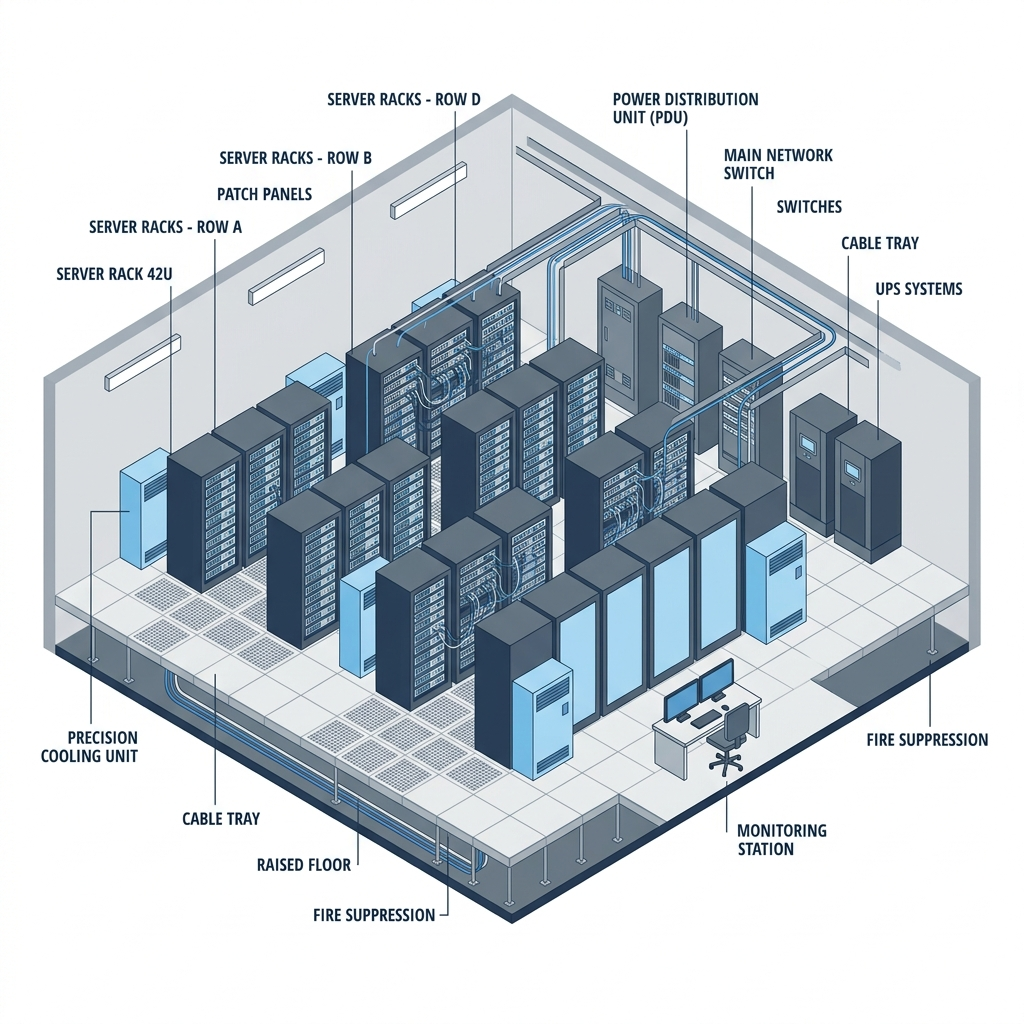
\includegraphics[width=0.8\textwidth]{images/datacenter_isometric.png}
    \caption{Illustrazione isometrica di un moderno datacenter ad alta densità.}
\end{figure}
\subsection{Dai Mainframe alla Bolla delle Dot-Com}
Storicamente, il calcolo centralizzato nasce negli anni '60 e '70 con i \textbf{Mainframe} (es. sistemi IBM): giganteschi armadi chiusi in stanze asettiche ("glass house") a cui gli utenti accedevano tramite terminali stupidi (green screen). In questa fase, il sistema era un blocco monolitico proprietario e altamente centralizzato.
Negli anni '80 e '90 si passa al modello \textbf{Client-Server}, con i server x86 (architettura aperta) distribuiti in semplici "sale server" aziendali, spesso ex ripostigli riadattati con un condizionatore commerciale e nessuna vera progettazione ingegneristica.
Alla fine degli anni '90, l'esplosione di Internet porta alla \textbf{bolla delle Dot-Com}: la necessità di scalare globalmente spinge le aziende ad affittare spazio (Colocation) in giganteschi edifici specializzati gestiti da telco e provider, per garantire l'accessibilità H24. Da qui nasce il vero e proprio concetto moderno di Datacenter.

\subsection{L'Era dell'Intelligenza Artificiale e la Top500}
Oggi si tratta di un'infrastruttura critica a livello nazionale, che richiede investimenti dell'ordine di centinaia di milioni, se non miliardi, di euro. 
L'esplosione dell'intelligenza artificiale (IA) ha portato all'era delle \textbf{AI Factories}: complessi industriali in grado di assorbire fino a 1-2 Gigawatt, l'equivalente di un'intera città.
La potenza di questi cluster è costantemente tracciata da due classifiche mondiali semestrali (nate nel 1993):
\begin{itemize}
    \item \textbf{Top500:} Misura le prestazioni assolute (benchmark di algebra lineare in PetaFLOPS).
    \item \textbf{Green500:} Misura l'efficienza energetica (GigaFLOPS per Watt), evidenziando il profondo \textbf{impatto ambientale} di queste strutture.
\end{itemize}

L'IA ha radicalmente alterato i paradigmi del passato: mentre nel Cloud computing tradizionale si sfrutta la virtualizzazione per massimizzare l'uso dell'hardware (normalmente inattivo per il 90\% del tempo), l'IA è il primo \textit{workload} che \textbf{satura integralmente l'hardware fisico}. Questo rende la virtualizzazione inutile nello stack AI e impone l'utilizzo di architetture hardware distribuite su decine di migliaia di GPU interconnesse.

\section{Fondamenti e Vincoli Fisici}
La costruzione di un datacenter moderno si scontra con limiti ingegneristici definiti \textbf{Hard Thresholds}: soglie fisiche oltre le quali non è possibile semplicemente "scalare" (ingrandire) una tecnologia, ma diventa necessario un ripensamento radicale.

\begin{warningbox}[Attenzione: Scale Up vs Scale Out]
\begin{itemize}
    \item \textbf{Scale Out:} aggiungere nuovi nodi o server per distribuire il carico.
    \item \textbf{Scale Up:} aumentare la capacità del singolo nodo (o, nel caso elettrico, del singolo cavo o edificio).
\end{itemize}
L'infrastruttura elettrica di un intero datacenter è costretta a operare in logica \textbf{Scale Up}: all'aumentare del consumo occorrono cavi in rame via via più spessi e costosi.
\end{warningbox}

\subsection{Pavimento Flottante}
\begin{figure}[H]
    \centering
    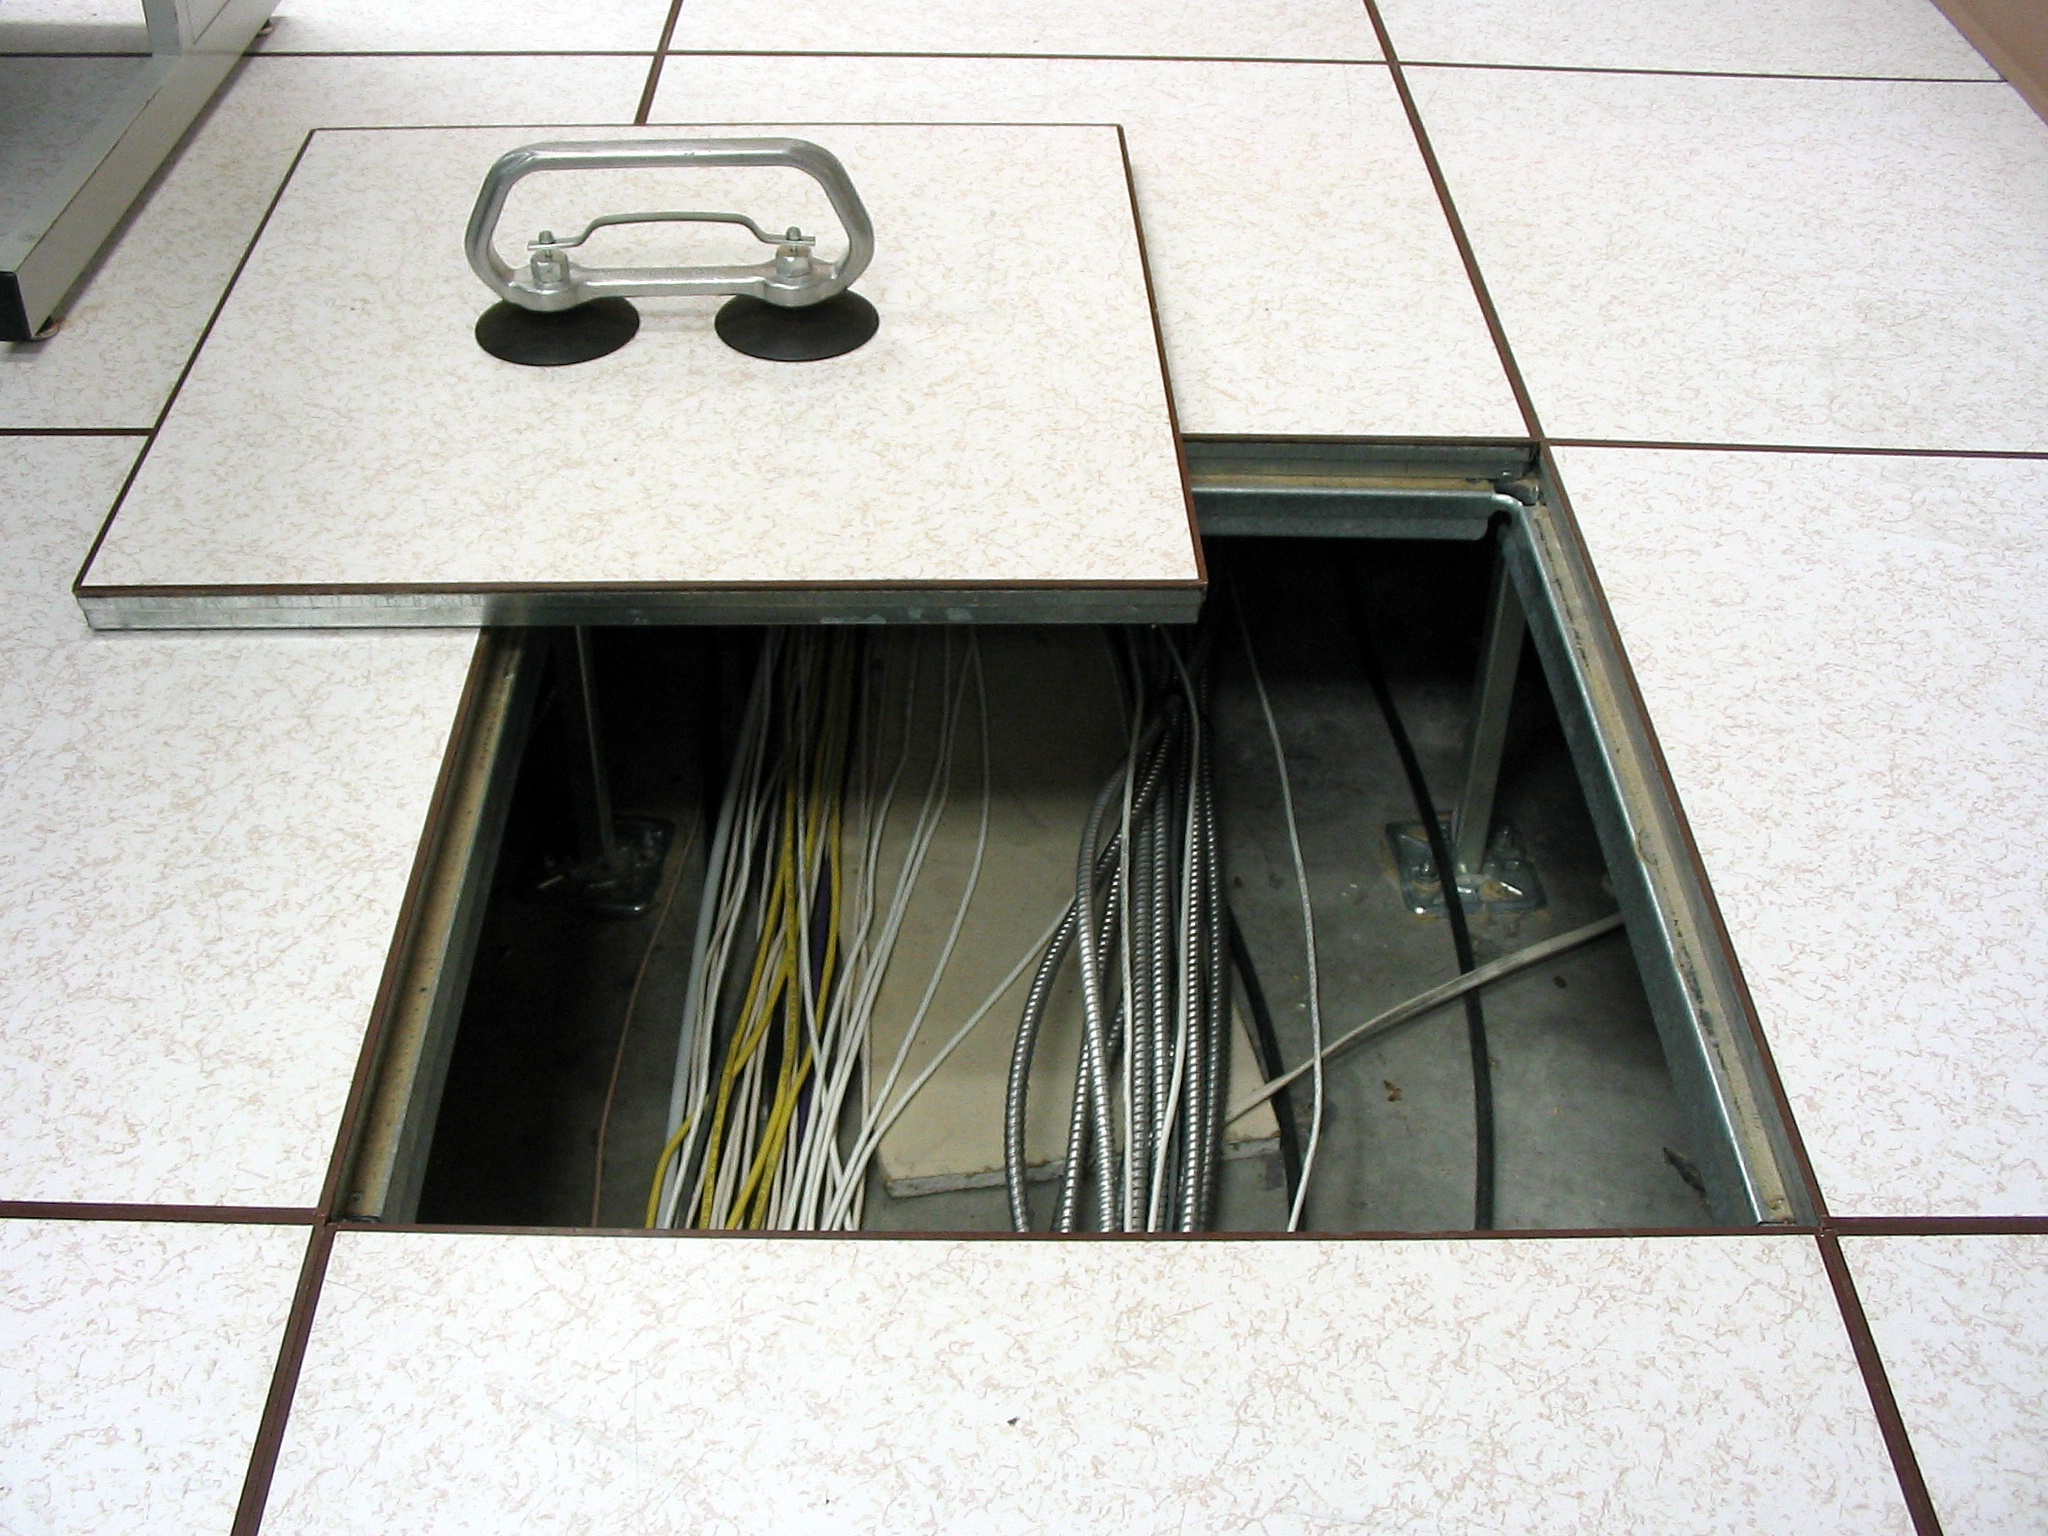
\includegraphics[width=0.7\textwidth]{images/raised_floor.jpg}
    \caption{Sollevamento di una piastrella dal pavimento flottante in un data center (Wikimedia Commons).}
\end{figure}
Una delle eredità ingegneristiche più diffuse è il \textbf{Floating Floor} (pavimento flottante). Costituito da pannelli sollevati su piedistalli metallici, nei moderni DC può reggere fino a 1.5 tonnellate per metro quadrato.
I due grandi vantaggi sono:
\begin{enumerate}
    \item \textbf{Gestione cavi:} passaggio ordinato dell'infrastruttura di cablaggio e tubazioni idrauliche.
    \item \textbf{Plenum per l'aria:} creazione di un condotto pressurizzato sotto il pavimento per distribuire l'aria fredda dal sistema di raffreddamento verso le griglie posizionate di fronte ai rack.
\end{enumerate}

\section{Raffreddamento e Gestione Termica}
A causa dell'estrema densità di calore, dovuta all'elevato \textbf{TDP (Thermal Design Power)} dei nuovi processori (che raggiungono il Kilowatt per singola GPU), il controllo termico è diventato l'aspetto più critico del design. 
La temperatura estrema può fondere i componenti in silicio; l'interruzione del sistema di raffreddamento, unita al tentativo delle ventole dei server di spingere aria, causa aumenti termici esponenziali che possono danneggiare l'intera stanza in pochissimi minuti.

\subsection{L'Architettura ad Aria: Sistemi CRAC e Flussi}
\begin{figure}[H]
    \centering
    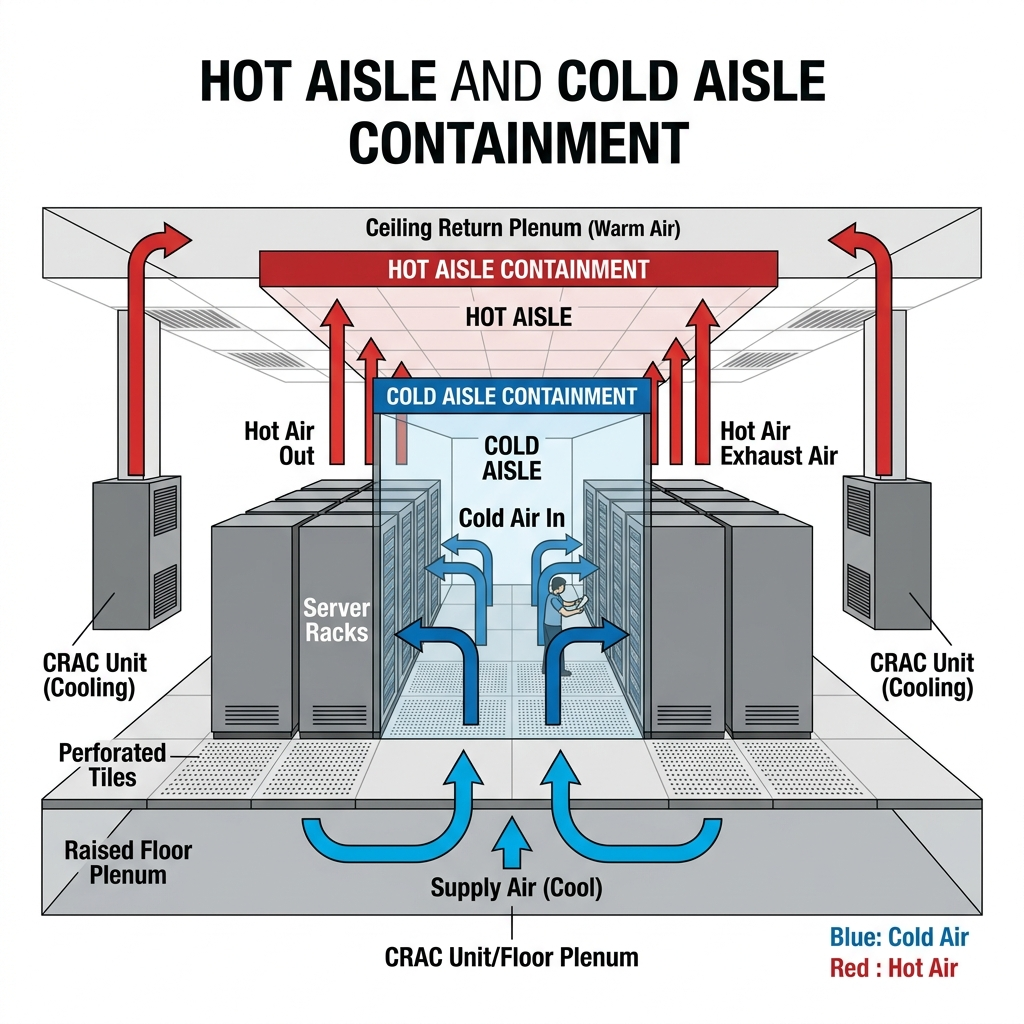
\includegraphics[width=0.8\textwidth]{images/aisle_containment.png}
    \caption{Schema del flusso d'aria: contenimento del corridoio freddo (Cold Aisle Containment) e corridoio caldo.}
\end{figure}
I sistemi \textbf{CRAC (Computer Room Air Conditioning)} si basano sul pavimento flottante e sul principio della rigorosa separazione tra \textit{Cold Aisle} (corridoio freddo) e \textit{Hot Aisle} (corridoio caldo). 
Il flusso dell'aria segue un percorso preciso: le unità CRAC immettono aria ghiacciata pressurizzata nel \textit{plenum} (lo spazio sotto il pavimento flottante). L'aria fuoriesce dalle grate forate esattamente di fronte ai rack (Cold Aisle). Le ventole dei server risucchiano l'aria frontalmente, raffreddano i dissipatori interni, ed espellono l'aria rovente dal retro nel corridoio caldo (Hot Aisle), dove sale verso il soffitto per tornare ai CRAC ed essere raffreddata nuovamente tramite scambiatori di calore ad acqua (Chiller).

\begin{tipbox}[Regola Aurea]
Mai mescolare l'aria calda e l'aria fredda. Se i flussi si mescolano, l'efficienza crolla e le CPU rischiano il \textit{thermal throttling}. Per questo si usano porte a vetri e tettucci chiusi per creare sistemi di \textbf{contenimento fisico} dei corridoi.
\end{tipbox}

Tuttavia, l'aria è un pessimo conduttore termico. Per carichi elevati (Rack oltre i 15-20 kW, per non parlare dei moderni rack AI da 200 kW), i sistemi CRAC ad aria sono insufficienti.

\subsection{Liquid Cooling}
Il raffreddamento a liquido è oggi uno standard di fatto per l'high performance computing (HPC):
\begin{itemize}
    \item \textbf{Direct-to-Chip:} placche di rame raffreddate ad acqua poste direttamente a contatto con CPU, GPU e RAM. Rimuove la necessità di ventole ad alta velocità.
    \item \textbf{Waterless Cooling:} utilizzo di fluidi dielettrici (es. glicole) in tubazioni. In caso di sversamento, non causano cortocircuiti.
    \item \textbf{Immersion Cooling:} immersione completa della scheda madre in olio minerale. Elimina ogni punto di calore localizzato (hot-spot), ma rende la manutenzione complessa e costosa.
\end{itemize}

\section{L'Efficienza Energetica (PUE)}
L'efficienza di un datacenter si misura con un valore adimensionale standard, il \textbf{PUE (Power Usage Effectiveness)}:
\[
PUE = \frac{\text{Total Facility Power}}{\text{IT Equipment Power}}
\]
Più il PUE si avvicina a 1, maggiore è l'efficienza (significa che non si sta sprecando energia per raffreddare). I migliori data center odierni hanno un PUE annuo attorno a 1.15 - 1.20.

\section{Sicurezza e Continuità}
La progettazione logica segue la cosiddetta \textbf{CIA Triad}:
\begin{itemize}
    \item \textbf{C}onfidentiality (Riservatezza)
    \item \textbf{I}ntegrity (Integrità)
    \item \textbf{A}vailability (Disponibilità)
\end{itemize}

L'approvvigionamento elettrico è vitale. La distribuzione avviene seguendo una rigorosa catena:
Dalla rete esterna in alternata (AC), si passa agli \textbf{UPS (Uninterruptible Power Supply)} industriali (basati su enormi batterie e sistemi a molla precompressa per scambi istantanei) che stabilizzano la corrente e prevengono micro-interruzioni. Dagli UPS si arriva alle \textbf{PDU (Power Distribution Unit)} gerarchiche, fino ai server che internamente convertono l'AC in corrente continua (DC).

La necessità di resilienza estrema si scontra con limiti pratici e geografici. La collocazione dei data center deve infatti tener conto di variabili critiche quali rischio sismico, escursioni termiche, accesso immediato alla rete di trasmissione in altissima tensione e obblighi normativi imposti dal GDPR.

\chapter{Cablaggio, Switching e Fabric di Rete}

\section{Il Mezzo Fisico: Rame e Fibra Ottica}
La rete è il sistema vascolare del datacenter. L'evoluzione della densità di traffico ha segnato il progressivo abbandono del rame a favore della fibra ottica.

\subsection{Cavi in Rame ed Ethernet}
Storicamente, i data center si basavano pesantemente sul rame (es. i vecchi cavi \textbf{Cat 5} o Cat 5e che limitavano le velocità a 100 Mbps o 1 Gbps). I limiti fisici del rame (diafonia e attenuazione del segnale) e la necessità di gestire un preciso \textit{pin-out} per l'allineamento dei contatti hanno reso sempre più complessa l'evoluzione. 
Oggi, il tradizionale cavo in rame (standard Ethernet con connettore RJ45) è confinato al limite pratico dei \textbf{10 Gbps (Cat 6A)}. Andare oltre con standard come Cat 7 o Cat 8 risulta impraticabile: i cavi diventano spessi, rigidi e difficili da gestire (il cosiddetto \textit{cable management} è vitale, poiché un cablaggio disordinato blocca il flusso d'aria e distrugge l'efficienza termica del rack).

\subsection{Fibra Ottica e Transceiver}
\begin{figure}[H]
    \centering
    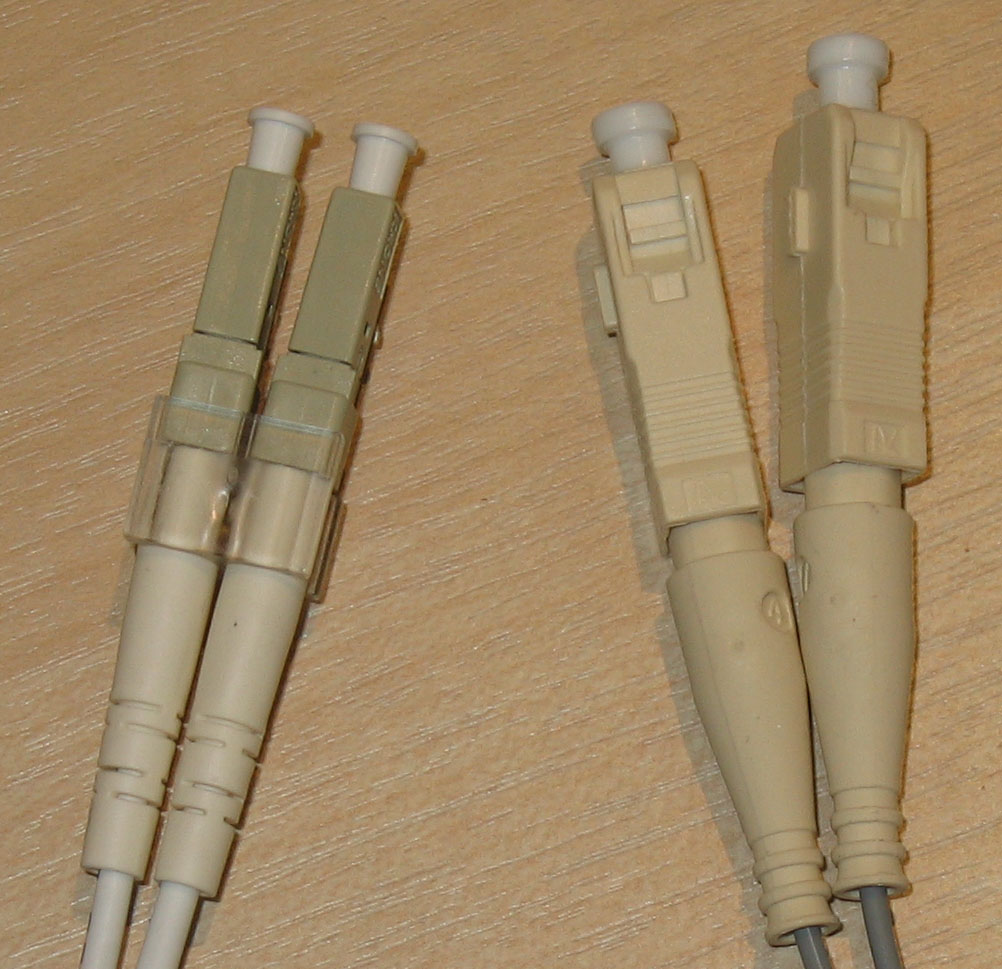
\includegraphics[width=0.6\textwidth]{images/fiber_connectors.jpg}
    \caption{Connettori ottici in fibra (LC e SC a confronto).}
\end{figure}
La trasmissione ottica azzera la dissipazione termica e aumenta vertiginosamente la banda, ma richiede l'uso di \textbf{transceiver} (moduli hot-swappable) per convertire il segnale elettrico in ottico. L'evoluzione di questi moduli ha definito le velocità del datacenter:
\begin{itemize}
    \item \textbf{SFP28:} Standard per porte server a 25 Gbps (singola lane).
    \item \textbf{Famiglia QSFP (Quad SFP):} Usa 4 lane interne. Include QSFP+ (40G), \textbf{QSFP28} (100G, standard per uplink), fino ai moderni \textbf{QSFP56} (200G) e \textbf{QSFP-DD} (fino a 800G).
\end{itemize}
Il salto prestazionale oltre i 100G non è avvenuto aggiungendo cavi, ma cambiando modulazione del segnale da \textbf{NRZ} (1 bit per simbolo) a \textbf{PAM4} (2 bit per simbolo, raddoppiando la banda alla stessa frequenza). I moduli utilizzano codici colore standardizzati incisi sul corpo (es. blu per monomodale, nero/grigio per multimodale).

Le fibre si dividono in due grandi famiglie:
\begin{itemize}
    \item \textbf{Multimodale (OM):} core più largo (50 $\mu$m), permette più rimbalzi dei fotoni. Ha distanze operative brevi (fino a $\sim$100-300 m) ma costi inferiori. È lo standard dominante \textit{all'interno} del datacenter.
    \item \textbf{Monomodale (OS):} core sottilissimo (9 $\mu$m), permette un unico percorso rettilineo. Ideale per collegamenti metropolitani a lungo raggio (fino a 40 km).
\end{itemize}

\section{Architettura interna degli Switch}
\begin{figure}[H]
    \centering
    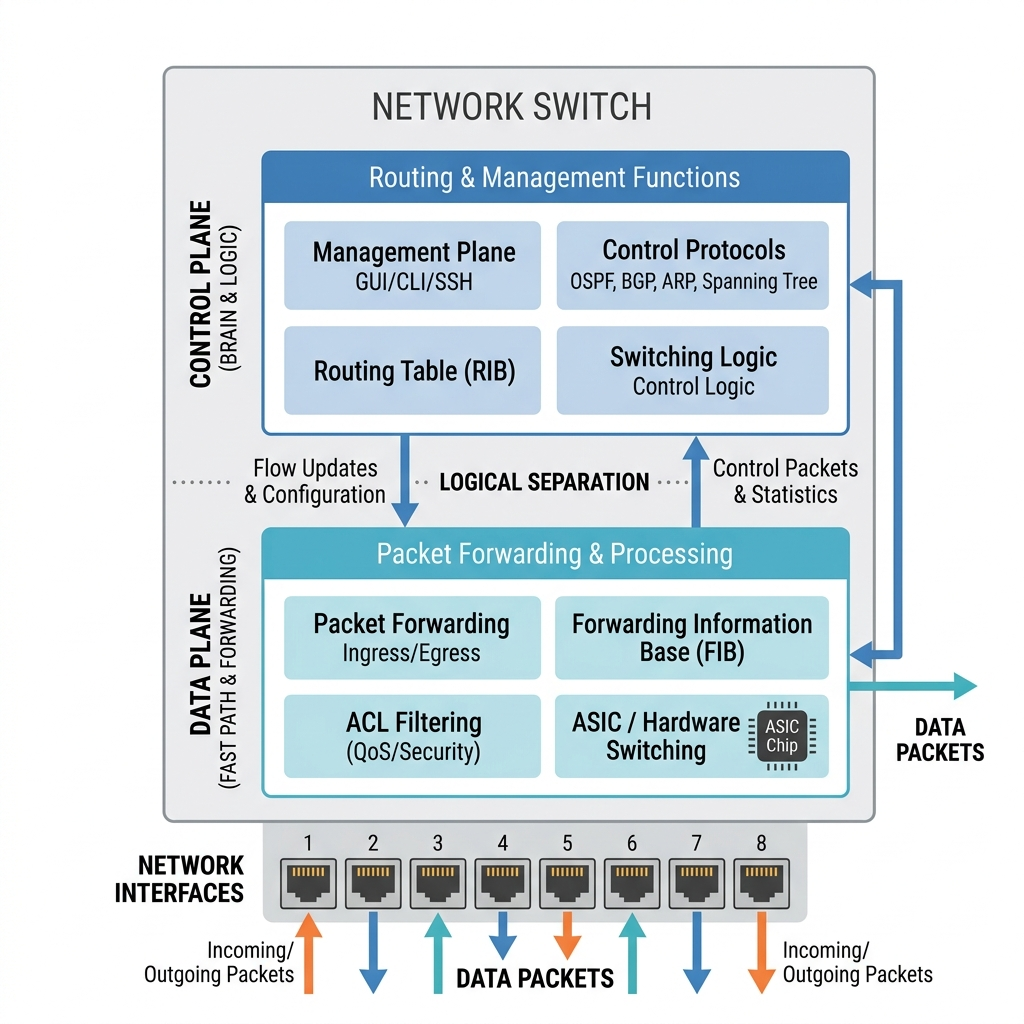
\includegraphics[width=0.7\textwidth]{images/network_planes.png}
    \caption{Architettura logica: separazione tra Control Plane e Data Plane in un dispositivo di rete.}
\end{figure}
In passato, l'architettura di rete dominante si basava su enormi \textit{chassis modulari} proprietari (es. i grandi switch core di Cisco), costosi e difficili da scalare gradualmente. Lo switch moderno, spinto dalle esigenze iperscalabili del cloud, ha abbandonato gli chassis a favore del \textbf{Fixed Form Factor} (1U o 2U), spesso definito \textit{White-box switch}.

\subsection{Software-Defined Networking (SDN) e SONiC}
\begin{figure}[H]
    \centering
    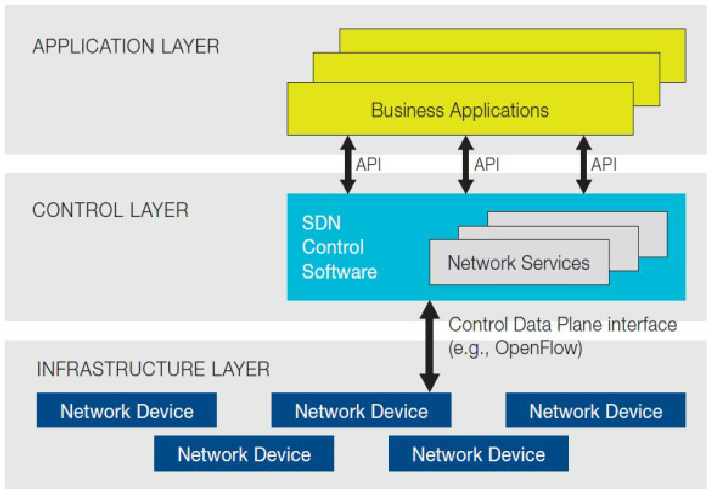
\includegraphics[width=0.7\textwidth]{images/sdn.png}
    \caption{Modello SDN: l'intelligenza di rete viene astratta dall'infrastruttura fisica sottostante.}
\end{figure}
La grande rivoluzione è stata la separazione concettuale in due piani:
\begin{enumerate}
    \item \textbf{Data Plane (Piano Dati):} hardware dedicato (spesso ASIC commodity, es. chip Broadcom) che si occupa di inoltrare pacchetti (\textit{forwarding}) a velocità \textit{line-rate}. Gli switch moderni sono \textit{non-blocking}, ovvero capaci di inoltrare traffico su tutte le porte simultaneamente senza colli di bottiglia.
    \item \textbf{Control Plane (Piano di Controllo):} un vero e proprio computer (spesso con CPU x86 e sistema operativo Linux) che gestisce la logica di rete (routing come BGP, policy, ecc.).
\end{enumerate}
\begin{figure}[H]
    \centering
    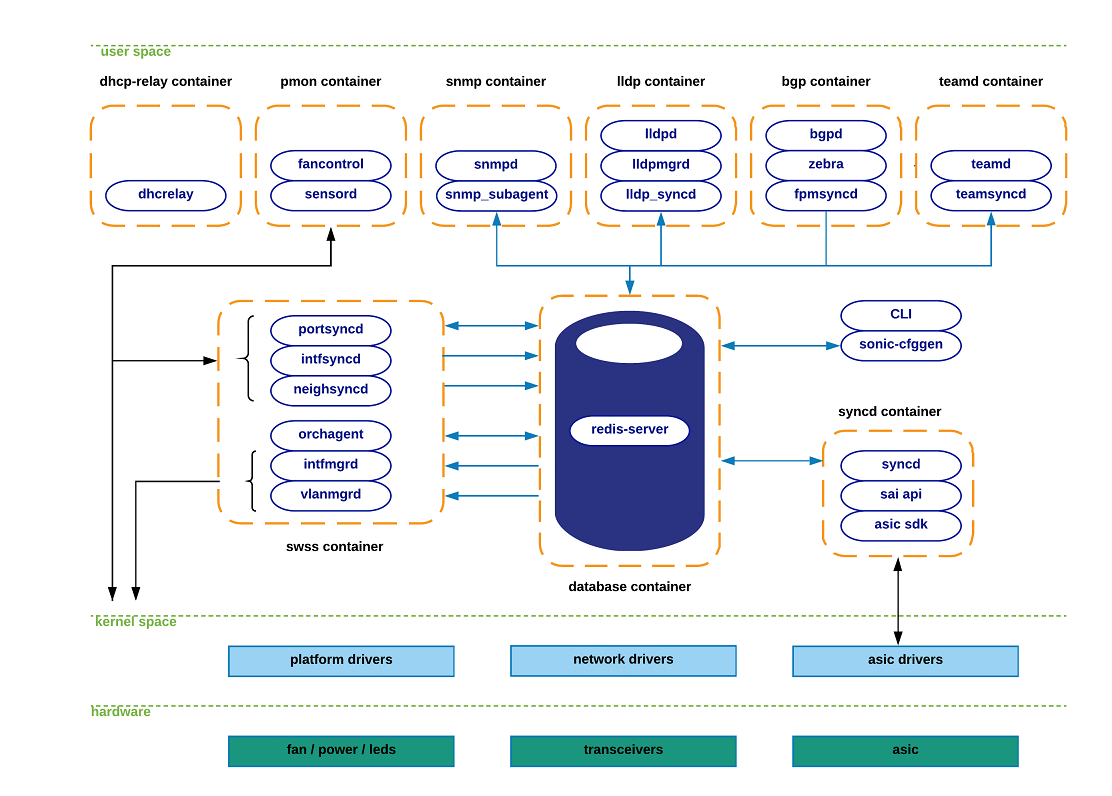
\includegraphics[width=0.7\textwidth]{images/sonic.png}
    \caption{Architettura SONiC: ogni funzione di rete gira nel proprio container Docker comunicando tramite Redis.}
\end{figure}
La disaggregazione hardware-software ha portato alla nascita di Sistemi Operativi di Rete (NOS) open source come \textbf{SONiC} (Software for Open Networking in the Cloud, creato da Microsoft). Avviato tramite il bootloader ONIE, SONiC tratta lo switch come un server standard, eseguendo ogni demone di routing all'interno di \textit{container Docker} isolati.

\section{Topologie di Rete: Dal 3-Tier allo Spine-and-Leaf}
Storicamente, i datacenter adottavano una topologia \textbf{3-tier} (Access, Distribution, Core), ottimizzata per il traffico \textbf{Nord-Sud} (client-server). 
I collegamenti ridondanti creavano inevitabilmente loop fisici. Se un pacchetto broadcast iniziava a ciclare, innescava un catastrofico \textbf{Broadcast Storm} in grado di paralizzare l'intero datacenter in pochi secondi. Per evitarlo si utilizzava il protocollo \textbf{STP (Spanning Tree Protocol)}, che disabilitava preventivamente i link fisici ridondanti. I difetti dell'STP erano molteplici: enormi sprechi di banda (fino al 50\% dei cavi posati rimaneva dormiente) e lenti tempi di convergenza in caso di guasto (i ricalcoli della topologia bloccavano momentaneamente il traffico).

Oggi, l'esplosione dei microservizi, del cloud e dell'IA ha reso assolutamente dominante il traffico \textbf{Est-Ovest} (server-to-server). La topologia standard dei moderni data center è diventata la \textbf{Spine-and-Leaf} (derivata dalle reti di \textit{Clos}):

\begin{figure}[H]
    \centering
    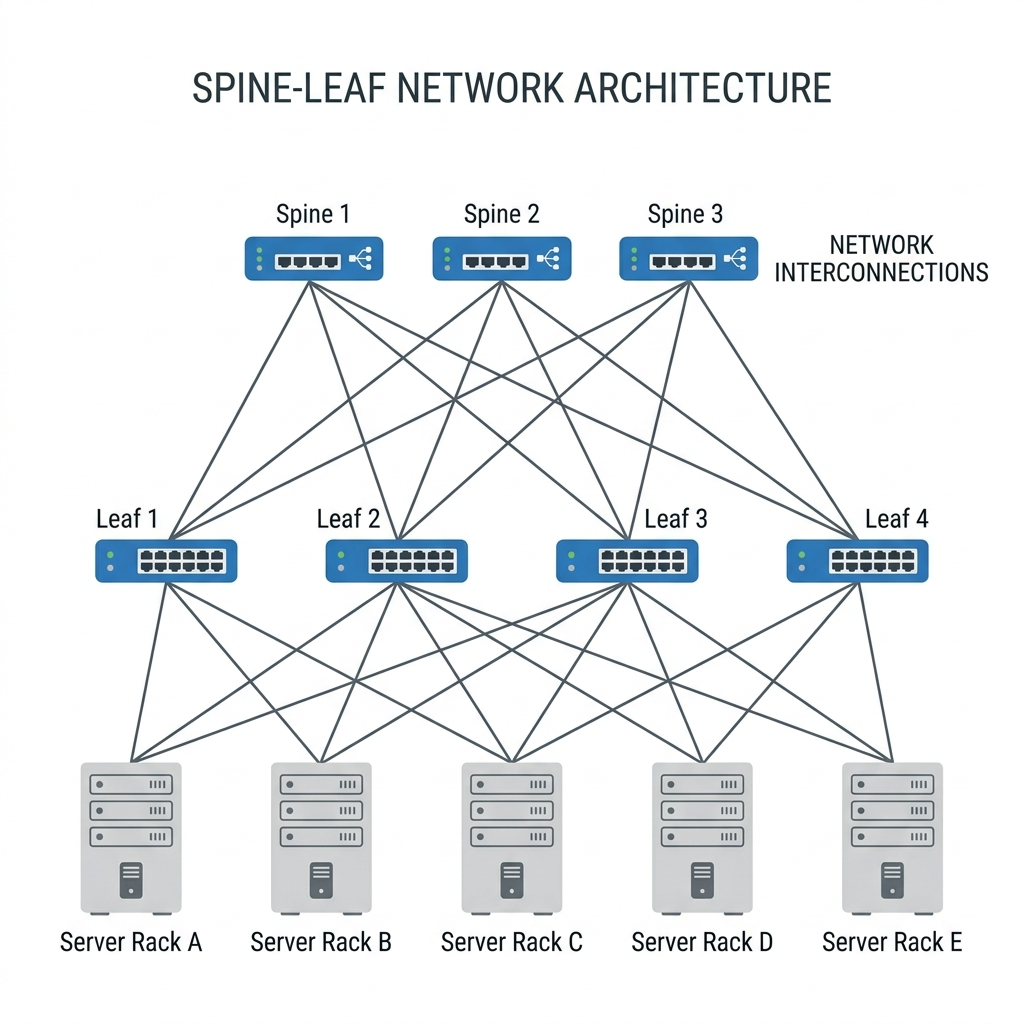
\includegraphics[width=0.8\textwidth]{images/spine_leaf_arch.png}
    \caption{Architettura Spine-Leaf: connessione Full-Mesh tra livello Leaf e livello Spine.}
\end{figure}

L'architettura si sviluppa su due livelli fisici rigorosi:
\begin{itemize}
    \item \textbf{Leaf Layer (Accesso):} Costituito dagli switch ToR (Top-of-Rack). I server fisici si collegano \textit{solo} a questi switch. A loro volta, gli switch Leaf \textbf{non sono mai collegati tra loro}.
    \item \textbf{Spine Layer (Backbone):} Il livello centrale di aggregazione. Ogni singolo switch Leaf possiede almeno un collegamento uplink in fibra verso \textbf{ogni} singolo switch Spine (creando una configurazione \textit{Full-Mesh} tra i due livelli). Anche gli switch Spine \textbf{non si parlano mai direttamente tra di loro}.
\end{itemize}

\begin{tipbox}[Vantaggi e Oversubscription]
\begin{itemize}
    \item \textbf{Latenza Deterministica:} Ogni server comunica con un qualsiasi altro server impiegando esattamente lo stesso numero di salti (1 hop logico: \textit{leaf $\rightarrow$ spine $\rightarrow$ leaf}).
    \item \textbf{ECMP (Equal-Cost Multi-Path):} Senza i tradizionali loop fisici, l'STP viene sostituito dal routing L3. Il traffico viene bilanciato uniformemente (load balancing) su \textit{tutti} gli uplink disponibili. Se uno switch Spine fallisce, la rete si degrada solo frazionalmente in banda, ma non si interrompe.
    \item \textbf{Oversubscription Ratio:} Il rapporto tra banda totale di downlink (verso i server) e uplink (verso gli Spine). Un tipico cloud usa rapporti 3:1. Gli ambienti HPC o AI esigono un rapporto \textbf{1:1} (detto \textit{Non-blocking}), garantendo che tutti i server possano trasmettere al massimo contemporaneamente senza colli di bottiglia.
\end{itemize}
\end{tipbox}

\section{Segmentazione e Virtualizzazione della Rete}
\subsection{VLAN (Virtual LAN)}
L'header Ethernet classico contiene un indirizzo MAC di destinazione (6 byte), un MAC sorgente (6 byte) e un campo EtherType (2 byte). Le VLAN (standard IEEE 802.1Q) permettono di suddividere una rete fisica in più domini di broadcast logici, inserendo un tag di 4 byte subito dopo il MAC sorgente. 
Questo tag 802.1Q include un campo TPID (che indica la presenza della VLAN) e un TCI, il quale a sua volta contiene 3 bit per la priorità (QoS) e \textbf{12 bit per l'identificativo VLAN (VID)}. Essendo l'ID VLAN lungo esattamente 12 bit, il limite teorico invalicabile è di \textbf{4094 reti} utilizzabili ($2^{12}-2$), un numero assolutamente insufficiente per i moderni cloud provider multi-tenant che devono ospitare centinaia di migliaia di reti isolate.

\subsection{VXLAN e Overlay}
Per superare la rigidità architetturale e il limite di 4096 reti delle VLAN tradizionali, il datacenter cloud moderno usa \textbf{VXLAN (Virtual eXtensible LAN)}. È un protocollo di \textit{overlay} (Mac-in-UDP) che incapsula interi pacchetti Layer 2 (Ethernet) all'interno di pacchetti di trasporto Layer 3 (UDP/IP). 
Questo innalza il limite a \textbf{16 milioni di reti virtuali isolate} (grazie a un identificativo VNI a 24 bit) e permette di creare domini di broadcast Layer 2 arbitrari su un'infrastruttura fisica di routing Layer 3. Ciò significa che due macchine virtuali possono credere di essere collegate allo stesso switch fisico (stessa subnet L2), anche se si trovano in due rack fisicamente distanti instradati in L3.

\section{Fabric ad Alte Prestazioni (HPC e AI)}
In contesti HPC e di addestramento AI, dove la computazione è pesantemente distribuita e sincronizzata, la latenza introdotta dallo stack TCP/IP Ethernet (tipicamente $\sim$70 $\mu$s) è inaccettabile.

In questi scenari domina \textbf{InfiniBand}, una rete che offre latenze di 1-3 $\mu$s. Il segreto è l'implementazione del protocollo \textbf{RDMA (Remote Direct Memory Access)}, che permette a un server di scrivere direttamente nella memoria RAM di un altro server scavalcando completamente l'intervento della CPU e del sistema operativo ricevente.
Oggi, RDMA è disponibile anche su reti Ethernet avanzate tramite il protocollo \textbf{RoCE} (RDMA over Converged Ethernet).

\begin{definitionbox}[Full Fat Tree]
Per evitare l'\textit{overbooking} (sovraccarico degli uplink) critico per l'HPC, si usa la topologia \textbf{Full Fat Tree}: una struttura non-bloccante in cui la larghezza di banda verso i livelli superiori è esattamente pari a quella dei livelli inferiori, garantendo comunicazioni senza strozzature.
\end{definitionbox}

\chapter{Storage: Architetture e Servizi}

\section{Evoluzione del Mezzo di Memorizzazione}
Lo storage rappresenta il secondo pilastro fondamentale di un datacenter, il luogo dove i dati persistono alla perdita di alimentazione (persistenza). La regola assoluta dello storage è una sola: \textbf{perdere i dati è il peccato imperdonabile}.

\subsection{Dal Nastro Magnetico all'HDD e all'SSD NVMe}
Storicamente, i primi datacenter utilizzavano \textbf{Nastri Magnetici (Tape)}: cartucce robotiche lente ma dalla capacità e densità enormi. Il nastro costringe ad un accesso sequenziale ai dati (non si può saltare alla fine senza "srotolare" tutto), ma è ancora oggi impiegato per il cold storage e i backup offline impenetrabili ai ransomware (Air-gap).

\begin{figure}[H]
    \centering
    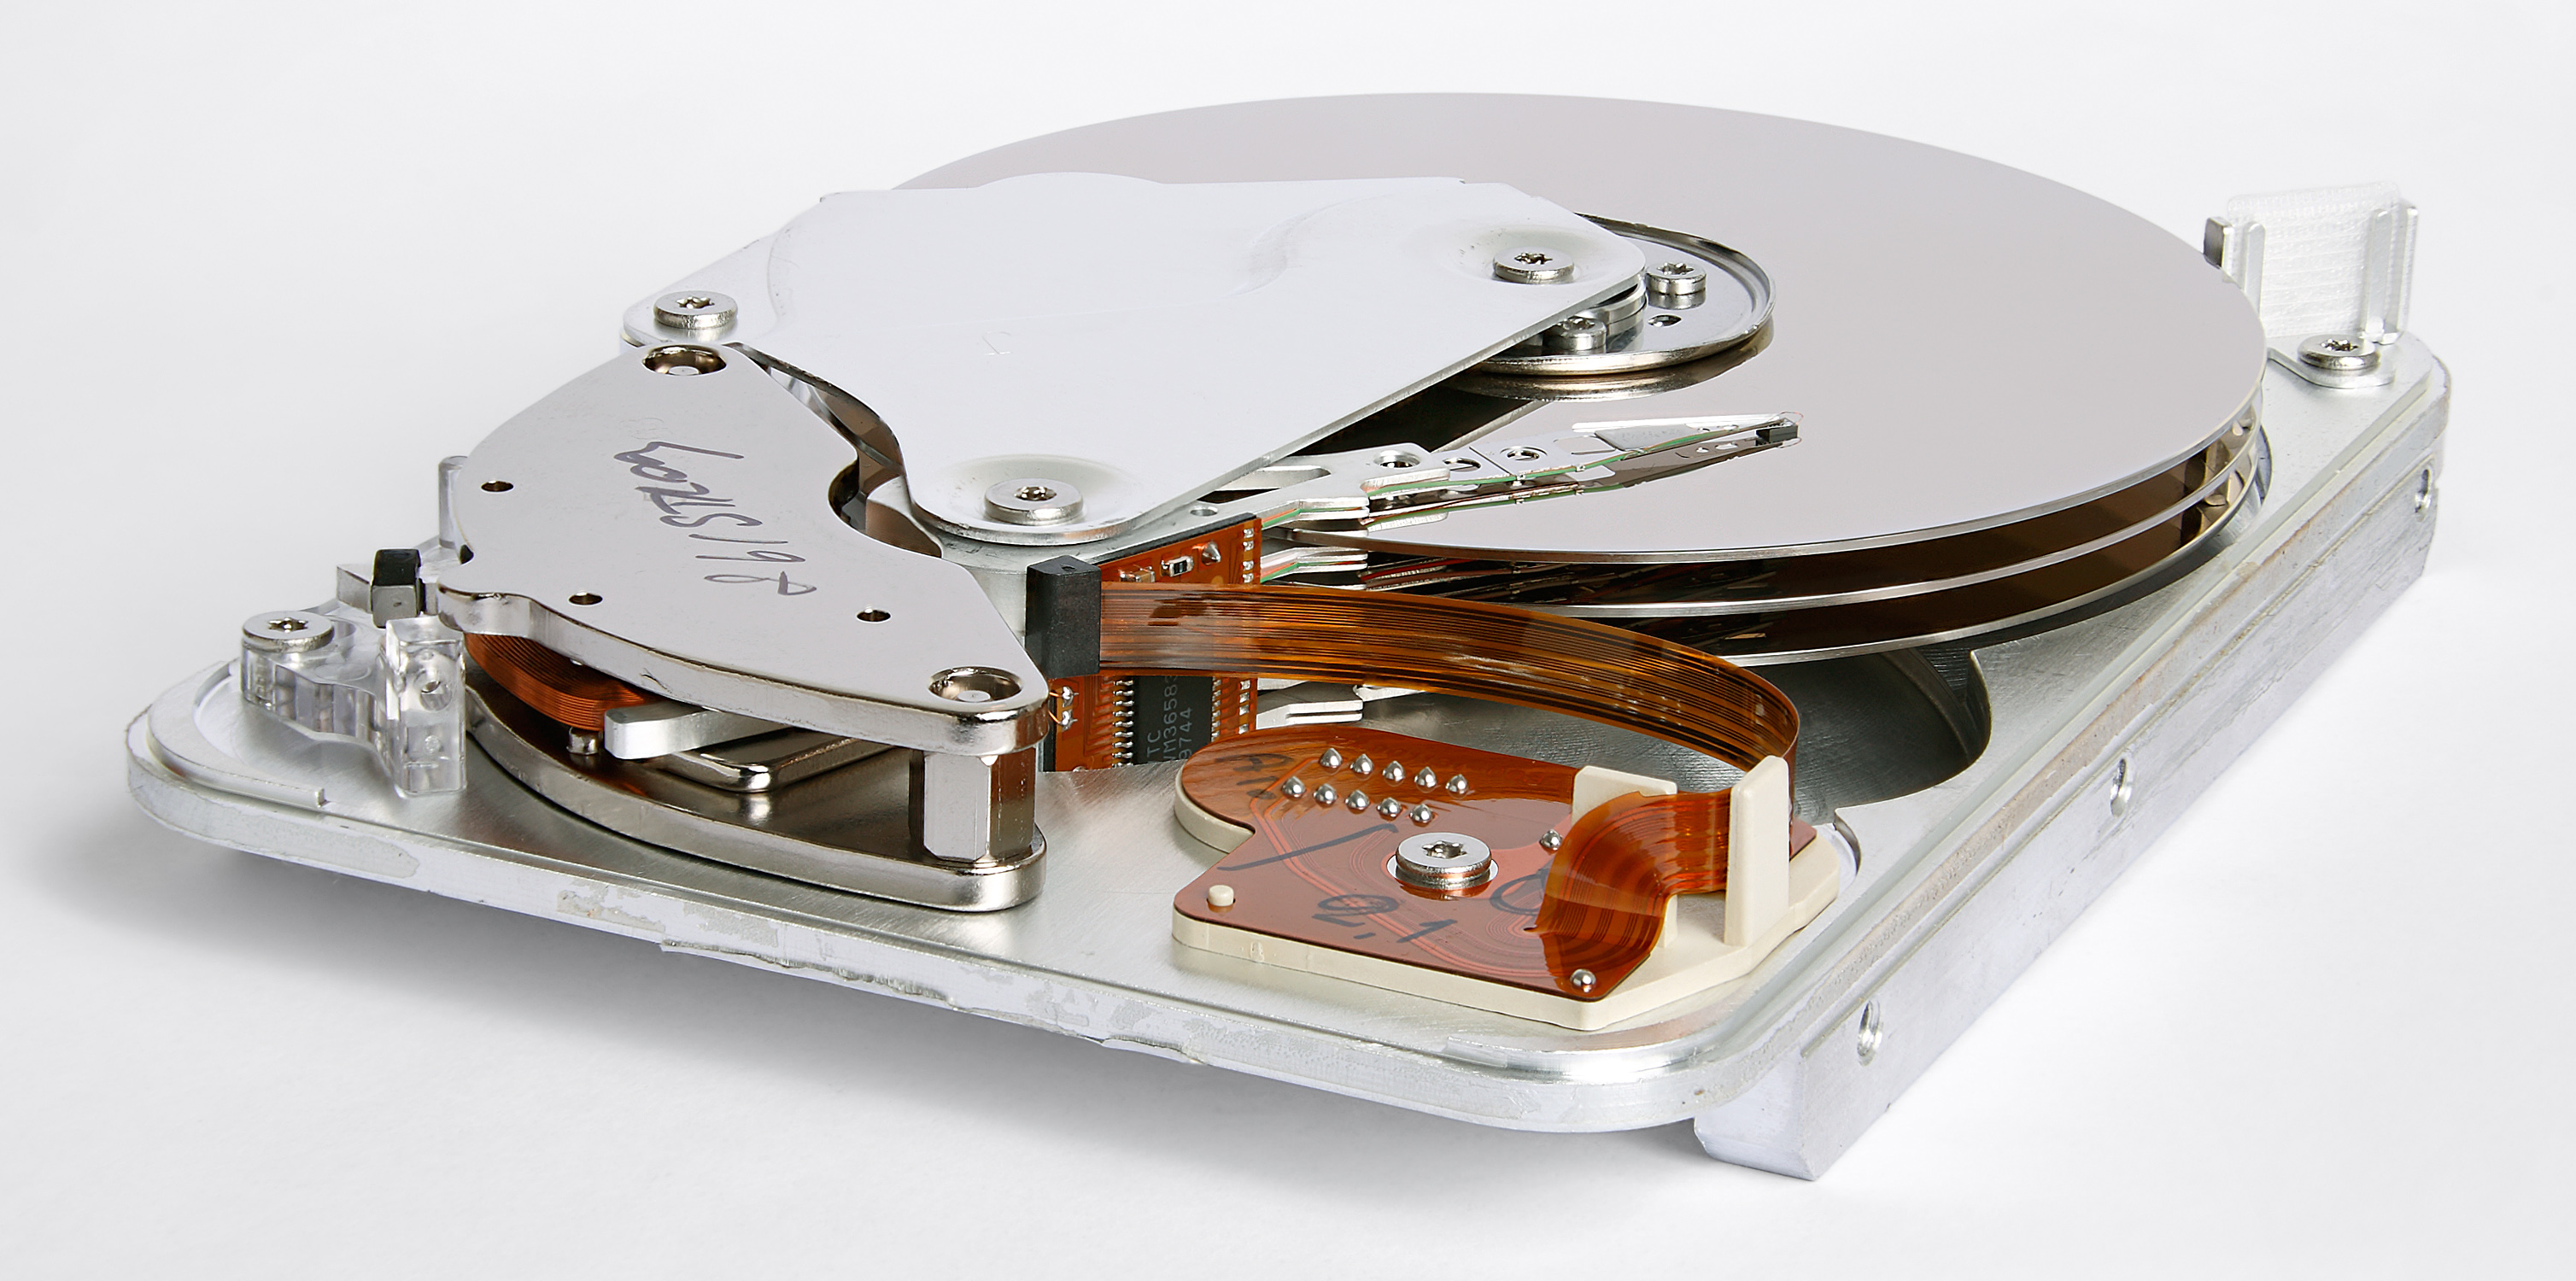
\includegraphics[width=0.6\textwidth]{images/hdd_inner.jpg}
    \caption{Interno di un Hard Disk Drive magnetico meccanico tradizionale.}
\end{figure}
Successivamente, si è passati agli \textbf{HDD (Hard Disk Drive)}, che offrono accesso casuale ai dati. Tuttavia, essi sono limitati da vincoli meccanici (rotazione dei piatti, tempo di \textit{seek} della testina), con latenze invalicabili di circa 3-5 ms. Le configurazioni storiche per i server usavano interfacce complesse in cascata (es. \textbf{SCSI}), oggi sostituite da protocolli SAS o SATA. Attualmente gli HDD sono relegati quasi esclusivamente all'archiviazione di massa a basso costo.

La transizione verso gli \textbf{SSD (Solid State Drive)} ha abbattuto la latenza a poche centinaia di microsecondi. Tuttavia, l'uso dei vecchi controller SATA si è rivelato rapidamente un collo di bottiglia. La rivoluzione successiva è stata l'introduzione dello standard \textbf{NVMe (Non-Volatile Memory Express)}, un protocollo che collega direttamente la memoria flash al bus \textbf{PCIe}, portando la latenza a $\sim$5-20 $\mu$s e il throughput a decine di GB/s.

\begin{tipbox}[Gerarchia della Memoria Moderna]
Con NVMe, il divario prestazionale tra DRAM (nanosecondi) e storage permanente (microsecondi) si è ridotto da 6 a soli 2 ordini di grandezza, permettendo architetture software impensabili prima, come database (es. RocksDB) che operano direttamente su storage senza pesanti strati di caching in RAM.
\end{tipbox}

\subsection{Celle NAND e Asimmetria}
A differenza della DRAM, la memoria NAND Flash presenta un'asimmetria intrinseca: le operazioni di lettura sono veloci, mentre le scritture richiedono un ciclo PE (Program/Erase) molto più lento. La densità dei bit per cella determina il tipo di SSD:
\begin{itemize}
    \item \textbf{SLC (Single-Level Cell):} 1 bit, altissima resistenza (100k cicli PE), altissimo costo.
    \item \textbf{MLC, TLC, QLC:} rispettivamente 2, 3 e 4 bit per cella. Costi decrescenti ma resistenza (endurance) e prestazioni in scrittura in rapido calo.
\end{itemize}

\subsection{Misure di Performance: IOPS, Latenza e Bandwidth}
Latenza e Bandwidth (throughput) da sole non sono sufficienti per caratterizzare le prestazioni di uno storage, poiché dipendono fortemente dal pattern di accesso (sequenziale o casuale). 
Una metrica fondamentale è l'\textbf{IOPS} (Input/Output Operations Per Second), ovvero il numero di operazioni di I/O completate in un secondo.
\begin{itemize}
    \item \textbf{Analogia del supermercato:} Gli IOPS rappresentano i clienti serviti al secondo, la latenza è il tempo impiegato in cassa per ogni cliente, e il parallelismo (le code) sono le casse aperte.
    \item La relazione base per una singola coda è: $\text{IOPS} \approx \frac{1}{\text{latenza}}$.
    \item Grazie alla natura asincrona dello storage, protocolli come NVMe (che supportano fino a 64.000 code parallele) permettono di scalare immensamente il throughput elaborando molte richieste simultaneamente.
\end{itemize}

\section{Aggregazione e Protezione: Il RAID}
Un singolo disco è un single point of failure inaccettabile. Si utilizza quindi il \textbf{RAID} (Redundant Array of Inexpensive Disks):
\begin{itemize}
    \item \textbf{RAID 0 (Striping):} Nessuna ridondanza, altissime prestazioni, rischio massimo.
    \item \textbf{RAID 1 (Mirroring):} Copia identica, perde il 50\% dello spazio.
    \item \textbf{RAID 5:} Ridondanza calcolata tramite funzione logica \textbf{XOR}. Tolleranza alla rottura di 1 solo disco. Se un secondo disco si rompe durante la fase di \textit{rebuild}, si perdono tutti i dati.
    \item \textbf{RAID 6:} Usa doppia parità, permettendo il fallimento simultaneo di \textbf{2 dischi}. È lo standard de facto nei datacenter odierni per via delle grandi capacità dei drive e dei lunghi tempi di rebuild.
\end{itemize}

\section{Architetture di Storage nel Datacenter}

\subsection{SAN (Storage Area Network)}
La SAN centralizza lo storage separandolo dai server, comunicando a livello di blocco (espone dischi grezzi, non file). I protocolli dominanti per questo fabric sono:
\begin{itemize}
    \item \textbf{Fibre Channel (FC):} Una rete fisicamente e logicamente separata dall'Ethernet standard. Richiede schede dedicate sui server, dette \textbf{HBA (Host Bus Adapter)}, e switch FC dedicati. Identifica i nodi non tramite MAC address, ma tramite indirizzi a 64 bit chiamati \textbf{WWN (World Wide Name)}.
    \item \textbf{iSCSI:} Alternativa economica che trasporta i comandi SCSI all'interno di normali pacchetti TCP/IP su rete Ethernet. Funziona tramite un'architettura client-server: il server host agisce da \textbf{iSCSI Initiator} (che richiede i blocchi), mentre lo storage array è l'\textbf{iSCSI Target} (che li fornisce). I nodi sono identificati tramite stringhe \textbf{IQN}.
    \item \textbf{FCoE (Fibre Channel over Ethernet):} Il tentativo di unificare le due reti. Incapsula i frame FC direttamente dentro l'Ethernet standard, eliminando la necessità di stendere cavi in fibra separati e riducendo il numero di switch, ma mantenendo il protocollo FC senza l'overhead del TCP/IP.
\end{itemize}

\begin{tipbox}[Sicurezza SAN: Zoning e Masking]
Per evitare che un server formatti per errore il disco (o intercetti i dati) di un altro server, si usano due barriere:
\begin{enumerate}
    \item \textbf{Zoning (Lato Rete):} Applicato sugli switch, crea zone hardware chiuse. Simile al concetto di VLAN nell'Ethernet, impedisce a due HBA che non sono nella stessa zona di comunicare o "vedersi" a vicenda.
    \item \textbf{LUN Masking (Lato Storage):} Lo storage array autorizza l'accesso a un disco logico (\textbf{LUN, Logical Unit Number}) esclusivamente allo specifico indirizzo WWN (per FC) o IQN (per iSCSI) del server proprietario.
\end{enumerate}
\end{tipbox}

\subsection{NAS (Network Attached Storage)}
Il NAS opera a un livello di astrazione più alto, connesso tramite rete Ethernet standard (protocolli NFS o SMB).
\begin{itemize}
    \item \textbf{Astrazione:} Espone un File System logico (\textit{file e directory}).
    \item \textbf{Limiti:} Maggiore latenza e impossibilità di usare la tecnica del \textit{memory mapping} in rete.
    \item \textbf{Casi d'uso:} File sharing, backup, documenti aziendali.
\end{itemize}

\subsection{Object Storage}
Sviluppato per gestire scalabilità a livello di Exabyte (es. Amazon S3). Abbandona cartelle e blocchi, utilizzando \textbf{oggetti} piatti allocati in \textit{bucket} e interrogabili tramite API REST.
Per garantire la scalabilità e distribuire i dati senza un collo di bottiglia centrale, utilizza algoritmi di routing come il \textbf{Consistent Hashing}. Ideale per dati statici e massivi, come dataset di Machine Learning o archivi medici.

\subsection{HCI (Hyper-Converged Infrastructure)}
Per decenni il mercato datacenter è stato dominato da grandi vendor che fornivano SAN e NAS hardware proprietari (es. i famosi array \textbf{EMC Symmetrix} o i \textbf{Filer NetApp}), apparati costosissimi e dal difficile scaling orizzontale. 
Per abbattere i costi e scalare linearmente, si è passati all'\textbf{HCI}, che trasforma lo storage SAN centralizzato in un approccio distribuito (*Scale-out*). Ogni server (nodo commodity x86) contiene CPU, RAM e dischi NVMe locali. Un livello software (Software-Defined Storage) raggruppa tutti i dischi locali di tutti i nodi e li presenta all'hypervisor come un'unica grande SAN virtuale condivisa.
\begin{tipbox}[Vantaggio dell'HCI]
\textbf{Data Locality:} Il software tenta sempre di scrivere/leggere i dati di una VM nel disco fisicamente residente nello stesso server che la esegue, azzerando il traffico di rete Nord-Sud e sfruttando al massimo la banda PCIe locale.
\end{tipbox}

\subsection{Storage per l'AI: Vector Database}
L'emergere dell'Intelligenza Artificiale generativa ha richiesto nuovi paradigmi di memorizzazione. La ricerca testuale classica era puramente \textit{sintattica} (come nel modello \textit{bag of words}), mentre i modelli neurali operano sulla \textit{semantica}.
\begin{itemize}
    \item \textbf{Embeddings:} Le reti neurali (LLM) trasformano testi, immagini o audio in vettori densi ad altissima dimensionalità (es. 3000 dimensioni). Questi vettori, chiamati \textit{embedding}, rappresentano il reale significato del dato in base al contesto (es. distinguono "Python" come linguaggio da "Python" come serpente).
    \item \textbf{Vector Database:} Sono una nuova generazione di database NoSQL progettati specificamente per immagazzinare e indicizzare questi enormi vettori. Per rispondere a una query, vettorializzano la domanda dell'utente e cercano i documenti semantici più simili calcolando la \textbf{distanza coseno} nello spazio vettoriale.
\end{itemize}
\begin{tipbox}[RAG: Retrieval-Augmented Generation]
I Vector Database sono il motore dell'architettura \textbf{RAG}, tecnica essenziale per limitare le "allucinazioni" delle AI. Prima di rispondere a un prompt, il sistema interroga il vector database, recupera i documenti aziendali realmente pertinenti, li inietta nel prompt e obbliga il LLM a formulare la risposta basandosi unicamente su quei fatti verificati.
\end{tipbox}

\section{Servizi Avanzati e Resilienza}

\subsection{Snapshot, Thin Provisioning e Replica}
\begin{itemize}
    \item \textbf{Thin Provisioning:} Permette di allocare logicamente più spazio agli utenti rispetto a quanto fisicamente presente nello storage, basandosi sul principio che raramente lo spazio allocato viene subito riempito (\textit{Overcommitment}). Il rischio intrinseco è esaurire fisicamente lo spazio se tutti gli utenti scrivono contemporaneamente, causando un blocco sistemico dei dischi.
    \item \textbf{Snapshot vs Clone:} La \textit{Snapshot} è una fotografia istantanea del volume che occupa inizialmente zero spazio aggiuntivo. Sfrutta il meccanismo del \textbf{Copy-on-Write (COW)}: congela i blocchi originali e alloca nuovi blocchi solo per le successive scritture. Se i dati originali si rompono, la snapshot è inservibile perché basata su puntatori condivisi. Un \textbf{Clone}, invece, è una copia fisica completa bit-a-bit (che impiega tempo e spazio) ed è totalmente indipendente.
    \item \textbf{Replica Sincrona/Asincrona:} Indispensabile per il Disaster Recovery. Nel caso di siti geografici vicini (max 300 km o 15ms di latenza round-trip), è possibile realizzare \textbf{Metro Cluster} con replica sincrona active-active.
\end{itemize}

\subsection{Backup vs Replica}
La \textbf{replica} è una copia speculare in tempo reale: protegge dai guasti hardware, ma propaga istantaneamente cancellazioni umane o attacchi ransomware. Il \textbf{backup} è un salvataggio point-in-time e sconnesso (offline) che permette il recupero.

Nel dimensionamento di un sistema di continuità aziendale due metriche sono fondamentali:
\begin{itemize}
    \item \textbf{RPO (Recovery Point Objective):} Quantità di dati che l'azienda è disposta a perdere (frequenza dei backup).
    \item \textbf{RTO (Recovery Time Objective):} Tempo massimo tollerabile per il ripristino dell'infrastruttura.
\end{itemize}

\begin{warningbox}[GDPR e Data Breach]
Secondo il GDPR, un \textit{data breach} non è solo il furto dei dati (perdita di \textit{confidenzialità}), ma include anche la perdita di \textit{integrità} (dati corrotti) e di \textbf{disponibilità} (dati integri ma non accessibili, ad esempio durante un attacco ransomware che cifra l'unico storage primario).
\end{warningbox}

\chapter{Compute e Virtualizzazione}

\section{Architettura Compute: CPU, GPU e NPU}
L'elaborazione dei dati (Compute) è il terzo pilastro del datacenter. L'evoluzione hardware moderna è guidata dalla fine della scalabilità lineare del singolo core (Legge di Moore) e dalla necessità di efficienza e specializzazione per carichi di lavoro legati all'Intelligenza Artificiale.

\subsection{Sostenibilità Energetica}
I datacenter consumano enormi quantità di energia elettrica e acqua. Le metriche di riferimento sono:
\begin{itemize}
    \item \textbf{PUE (Power Usage Effectiveness):} Rapporto tra energia totale consumata dal datacenter e quella effettivamente usata dai server. Il valore ideale è 1.0.
    \item \textbf{WUE (Water Usage Effectiveness):} Consumo idrico per kWh, critico nei datacenter che usano raffreddamento evaporativo (Torri di raffreddamento).
\end{itemize}

\subsection{Architettura CPU: Pipeline e Multi-Core}
Storicamente, per aumentare le prestazioni, si aumentava la frequenza di clock e si ottimizzava la \textbf{Pipeline delle istruzioni} (suddivisa classicamente nelle fasi: \textit{Instruction Fetch, Decode, Execute, Memory Access, Write-back}). Aumentando la profondità della pipeline (fino a 20+ stadi), si potevano eseguire più istruzioni sovrapposte nel tempo, ma gli errori di previsione dei salti (\textit{Branch Misprediction}) causavano lo stallo e lo svuotamento completo della coda ("bolle" nella pipeline), vanificando l'efficienza. 

Arrivati al limite fisico del calore dissipabile (Power Wall), si è passati al parallelismo Multi-Core. Per superare i colli di bottiglia della condivisione della RAM, le CPU moderne adottano architetture \textbf{NUMA (Non-Uniform Memory Access)}, in cui ogni processore ha un proprio banco di memoria locale ad accesso diretto rapido; l'accesso alla RAM degli altri processori avviene tramite interconnessioni esterne a latenza maggiore.

\textbf{Hyperthreading e SMT (Simultaneous Multithreading)}\\
Per ridurre al minimo i tempi morti (idle time) in cui un core attende dati dalla memoria, i progettisti hanno introdotto l'\textbf{Hyperthreading} (o SMT). Il trucco consiste nel duplicare solo le risorse "leggere" (come i registri e il program counter), mantenendo condivise le costose unità di calcolo fisico (ALU). Il sistema operativo vede \textbf{due core logici} per ogni core fisico: quando un thread è in stallo per un \textit{cache miss}, il core scambia istantaneamente contesto ed esegue le istruzioni dell'altro thread.
Sebbene eccellente per server web e database ad alto I/O, l'HT è \textbf{dannoso in ambito HPC} (High Performance Computing): se due thread devono fare calcolo intensivo matematico simultaneo, lotteranno aspramente per l'unica ALU condivisa, riducendo le performance generali. Nei supercomputer l'HT viene perciò disabilitato.

\begin{tipbox}[Overbooking e Memory Ballooning]
La virtualizzazione si fonda sull'\textbf{Overbooking} (sovra-allocazione logica delle risorse fisiche sottostanti). Oltre all'ovvio over-commit delle vCPU, si esegue overbooking pesante sulla RAM. Un meccanismo chiave è il \textbf{Memory Ballooning}: l'hypervisor inietta un driver-palloncino nel kernel del SO ospite. Se il server fisico sta esaurendo la vera RAM, l'hypervisor "gonfia" il palloncino. Il SO ospite crede di aver bisogno urgentemente di memoria interna, swappa i propri processi meno usati sul suo disco virtuale e restituisce la RAM vera al palloncino (e quindi all'hypervisor). L'hypervisor maschera inoltre enormi quantità di RAM tramite \textit{Memory Page Sharing} (es. KSM deduplica le pagine di sistema operativo identiche tra decine di VM Windows uguali).
\end{tipbox}

\begin{warningbox}[Vulnerabilità Side-Channel]
Condividere fisicamente la cache L1 e i buffer di esecuzione tra due thread apre la porta ad attacchi speculativi come \textbf{Spectre} o \textit{MDS}. Un thread malevolo può dedurre dati segreti del thread "fratello" misurando la latenza della cache. Per massima sicurezza, alcuni cloud provider disabilitano del tutto l'SMT.
\end{warningbox}

\begin{figure}[H]
    \centering
    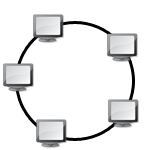
\includegraphics[width=0.6\textwidth]{images/ring_topology.png}
    \caption{Schema logico di una topologia Ring, storicamente usata per l'interconnessione interna dei core CPU.}
\end{figure}
\textbf{Interconnessione interna: Crossbar vs Bus}\\
A livello di interconnessione interna (die), le prime CPU multi-core usavano un \textit{Bus Condiviso}, che diventava subito un collo di bottiglia: solo un core alla volta poteva parlare. Oggi si utilizza la \textbf{Crossbar} (o una \textit{Mesh Network}): una matrice di interconnessione che permette a molteplici core di comunicare simultaneamente con banchi di memoria o I/O diversi senza intralciarsi, garantendo \textit{bisection bandwidth} completa.

Questo approccio reticolare si sposa perfettamente con l'architettura a \textbf{Tile (o Chiplet)}: i processori moderni non sono più un unico monolite di silicio prono a difetti, ma un mosaico di piccoli chip iperspecializzati (Compute Tile, I/O Tile) stampati con nodi differenti e incollati sullo stesso package, migliorando enormemente le rese produttive (yield) e abbassando i costi. Esempi concreti di questo approccio sono il fabric di interconnessione \textbf{AMD Infinity Fabric} per unire i chiplet nei processori EPYC, e le tecnologie di packaging avanzato 3D come \textbf{Intel EMIB e Foveros} (usate nelle architetture Meteor Lake e Sapphire Rapids) che impilano i die di silicio verticalmente.

\subsection{GPU e NPU: Il cambio di paradigma}
\begin{itemize}
    \item \textbf{CPU:} Ottimizzata per la \textit{minima latenza}. Pochi core molto complessi con esecuzione \textit{Out-of-Order} e grandi cache.
    \item \textbf{GPU:} Ottimizzata per il \textit{massimo throughput}. Migliaia di core semplici che eseguono lo stesso calcolo in parallelo (SIMT), ideale per l'addestramento dell'AI.
    \item \textbf{NPU (Neural Processing Unit):} Circuiti dedicati e specializzati esclusivamente nel calcolo tensoriale e inferenza AI a bassa precisione numerica e bassissimo consumo energetico.
\end{itemize}

\section{Architetture Server Fisici e BMC}
L'involucro fisico (form factor) dei server si è diversificato negli anni per rispondere a diverse esigenze di densità, potenza di calcolo e dissipazione termica.

\subsection{Server Rack (1U / 2U)}
\begin{figure}[H]
    \centering
    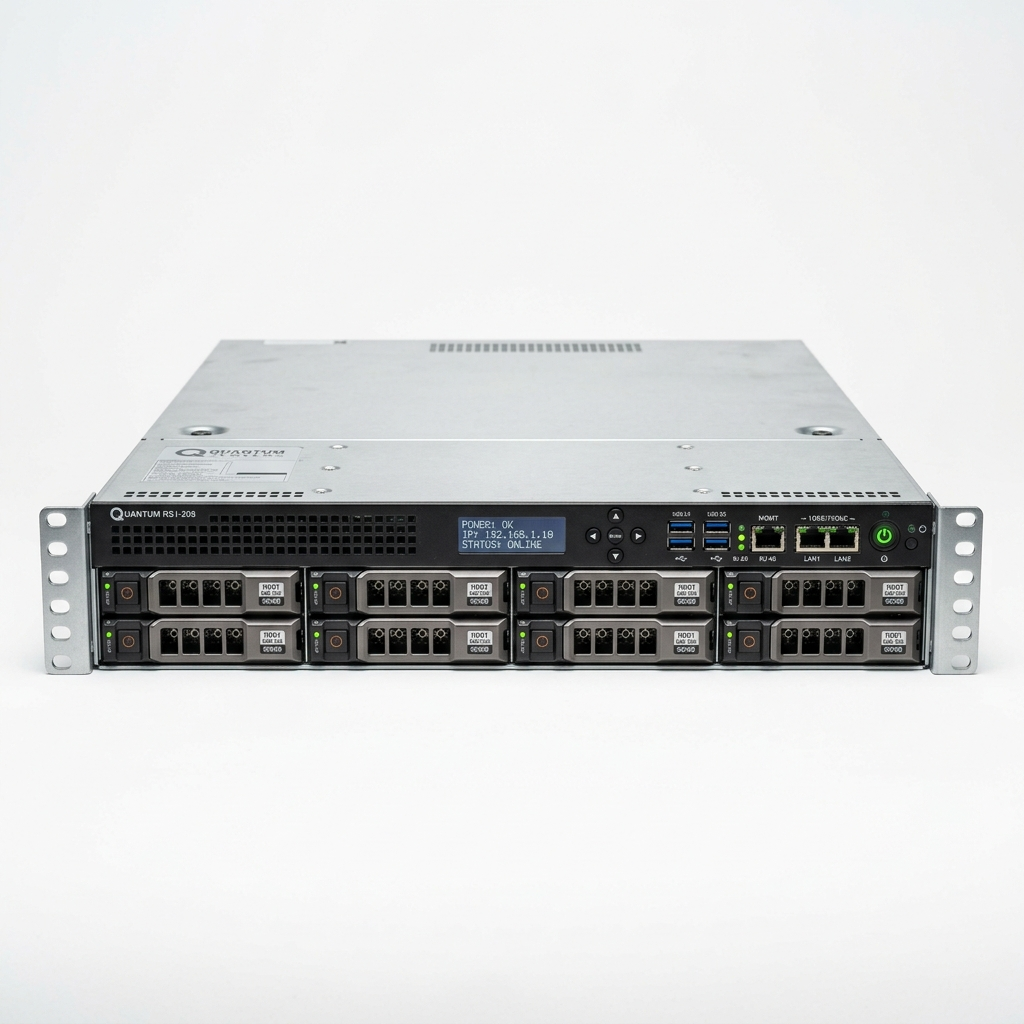
\includegraphics[width=0.7\textwidth]{images/rack_server_1u.png}
    \caption{Server Rack 1U standard con alloggiamenti per dischi frontali (hot-swap).}
\end{figure}
È il formato "general-purpose" più diffuso nei data center tradizionali. Un server rack è un computer completo e indipendente (dotato di propri alimentatori, ventole, CPU, RAM e dischi) racchiuso in uno chassis metallico standardizzato largo 19 pollici. L'altezza si misura in unità rack (U, circa 4,4 cm). Sono ideali per workload eterogenei, ma in grandi quantità richiedono un enorme lavoro di cablaggio singolo per ogni macchina (cavi di alimentazione e di rete separati per ogni singolo server).

\subsection{Blade Server}
\begin{figure}[H]
    \centering
    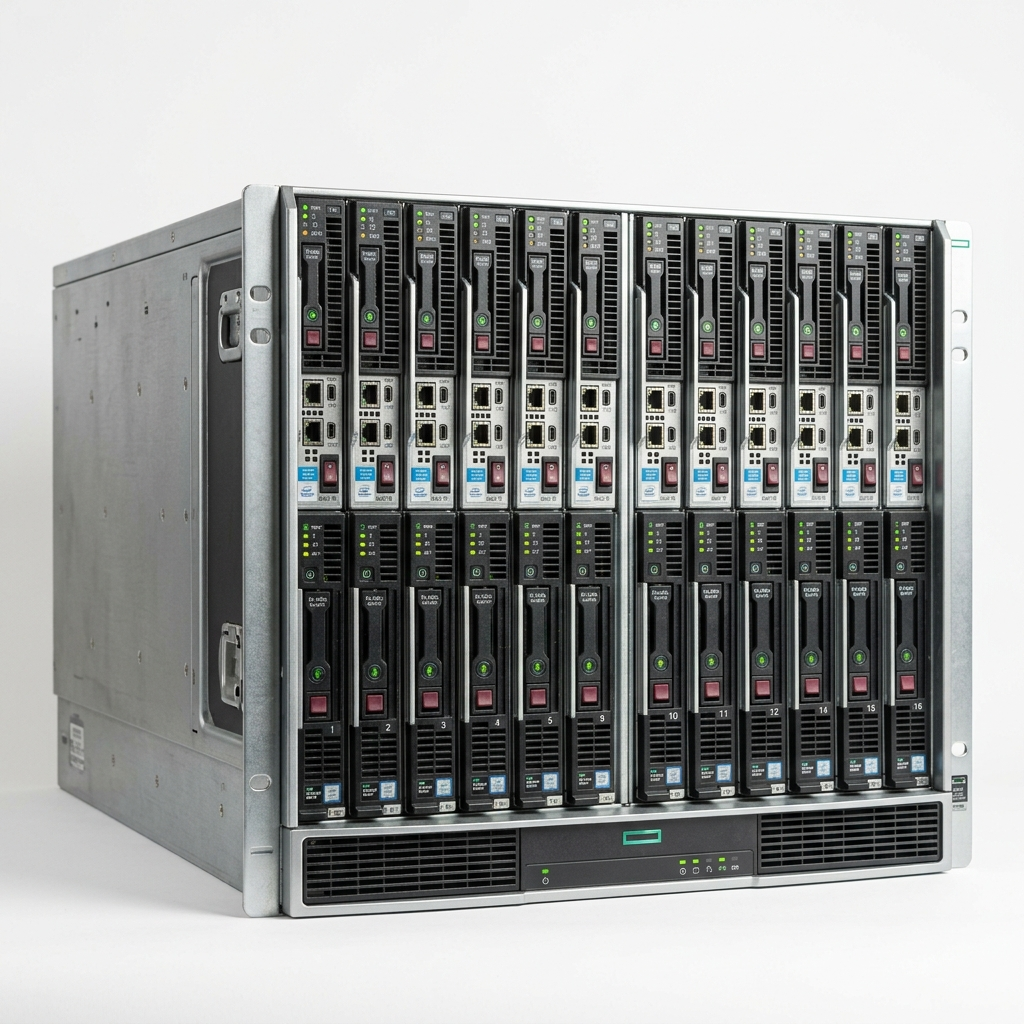
\includegraphics[width=0.7\textwidth]{images/blade_server.png}
    \caption{Chassis Blade System: decine di server-lama inseriti in un singolo modulo.}
\end{figure}
Progettati per ottenere l'altissima densità necessaria nei cluster di virtualizzazione. Un sistema Blade si divide in due componenti: lo \textbf{Chassis} (l'involucro esterno che fornisce alimentazione condivisa, mega-ventole e switch di rete integrati) e le \textbf{Lame} (i server veri e propri). La lama (Blade) è sottilissima perché contiene solo CPU, RAM e pochi dischi; non ha ventole o alimentatori propri. Inserendola nello chassis, si collega automaticamente al \textit{midplane} posteriore, azzerando quasi totalmente il disordine del cablaggio nel rack.

\subsection{Server HGX (AI GPU Server)}
\begin{figure}[H]
    \centering
    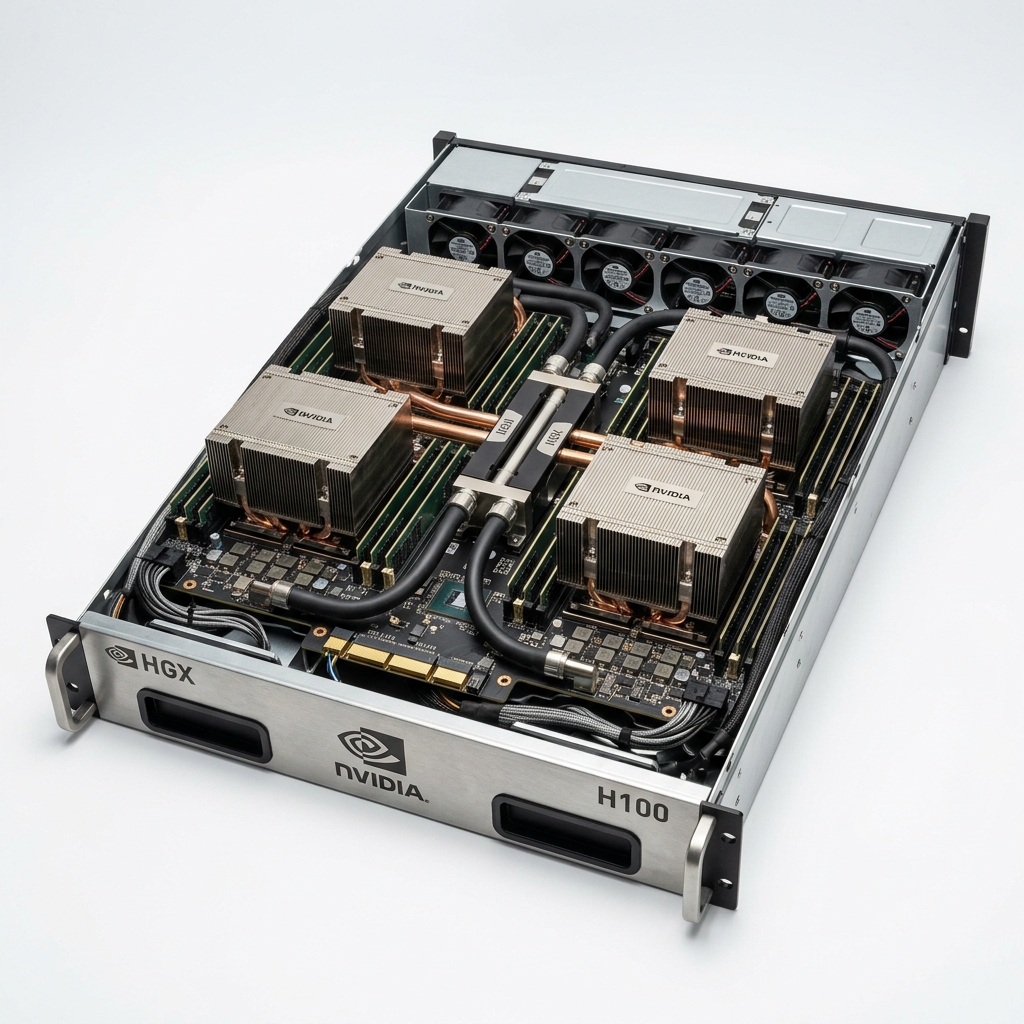
\includegraphics[width=0.7\textwidth]{images/hgx_gpu_server.png}
    \caption{Server HGX (aperto): GPU ad alte prestazioni coperte da enormi dissipatori metallici per gestire il calore estremo.}
\end{figure}
Con l'esplosione dell'intelligenza artificiale generativa, i normali server rack non sono più sufficienti. Un server HGX è una macchina immensa (spesso 4U o 8U, pesante oltre 100 kg) progettata esclusivamente attorno alle GPU (es. NVIDIA H100). Le GPU non sono più inserite come schede PCIe estraibili, ma sono saldate direttamente su una \textit{baseboard} proprietaria e interconnesse tramite bus dedicati (come NVLink) che scavalcano il collo di bottiglia del PCIe. Generano un calore spaventoso, rendendo spesso obbligatorio il passaggio al raffreddamento a liquido (\textit{Direct-to-Chip Liquid Cooling}).

\subsection{Standardizzazione Hyperscaler: Open Compute Project (OCP)}
Creato originariamente da Meta (Facebook) nel 2011, l'\textbf{OCP (Open Compute Project)} è un consorzio no-profit che pubblica le specifiche hardware open source per server e rack da datacenter. L'idea nasce da un'esigenza economica: i server tradizionali di brand contengono molte funzionalità estetiche o di gestione (frontalini in plastica, display, alimentatori ridondati per singolo server) inutili su scala hyperscaler.
Le specifiche OCP definiscono macchine essenziali (spesso prodotte direttamente da costruttori ODM taiwanesi come Quanta o Foxconn), permettendo risparmi enormi. Un'innovazione chiave dell'OCP è il design del rack: l'alimentazione non viene convertita in ogni singolo server, ma centralizzata a monte nel rack e distribuita ai server tramite busbar a 12V o 48V, aumentando l'efficienza energetica e la densità.

\begin{tipbox}[BMC (Baseboard Management Controller) e lo Standard Redfish]
Tutti i server di livello enterprise montano un \textbf{BMC} (es. iLO di HPE o iDRAC di Dell). Si tratta di un micro-computer indipendente inserito nella scheda madre, dotato di una porta di rete dedicata (\textit{out-of-band management}). Essendo alimentato separatamente, permette il controllo fisico del server (accensione, configurazione BIOS, console KVM virtuale) anche se il sistema operativo principale è bloccato o se il server è fisicamente spento.

\textbf{Redfish: L'API del Datacenter Moderno}\\
Storicamente, i BMC venivano gestiti tramite il protocollo IPMI, che col tempo si è rivelato insicuro e difficile da integrare. Per questo motivo, il consorzio DMTF ha introdotto \textbf{Redfish}, lo standard moderno per la gestione dell'infrastruttura.
\begin{itemize}
    \item \textbf{Come funziona:} Redfish espone tutti i parametri hardware tramite una \textbf{RESTful API} standard. Utilizza i protocolli del web moderno (HTTPS per la sicurezza) e restituisce i dati in formato \textbf{JSON} (OData), facilmente leggibile sia dagli umani che dagli script.
    \item \textbf{Cosa fa:} Permette di automatizzare su larga scala le operazioni più tediose. Tramite semplici script Python o strumenti come Ansible, si possono inviare richieste web (GET, POST, PATCH) per monitorare le temperature, aggiornare i firmware, modificare l'ordine di boot o riavviare un intero rack di server, indipendentemente dalla marca dell'hardware sottostante.
\end{itemize}
\end{tipbox}

\section{Virtualizzazione e Live Migration}
La virtualizzazione svincola il software dall'hardware fisico, permettendo a più Sistemi Operativi (Guest) di girare simultaneamente sullo stesso server fisico (Host). Il cuore di questo processo è l'\textbf{Hypervisor} (o Virtual Machine Monitor).

\subsection{L'Evoluzione dell'Hypervisor: Dai Ring CPU alla Virtualizzazione Hardware}
L'architettura x86 originale non era progettata per essere virtualizzata. Prevedeva quattro livelli di privilegio logici chiamati \textbf{Ring}, da Ring 0 (massimo privilegio, destinato al kernel del SO) a Ring 3 (spazio utente). 
In un ambiente virtualizzato, l'Hypervisor deve avere il controllo assoluto, quindi deve risiedere in Ring 0. Questo costringeva i sistemi operativi Guest a scalare in Ring 1 (modalità non privilegiata, definita \textit{Ring De-privileging}). Poiché i SO Guest non sapevano di essere virtualizzati, tentavano di eseguire istruzioni privilegiate (es. manipolazione hardware) che, fallendo, venivano intrappolate dall'Hypervisor. Quest'ultimo doveva tradurle ed emularle in tempo reale (tecnica della \textbf{Binary Translation}), causando un enorme e insostenibile overhead prestazionale.

Il problema è stato risolto nel 2005 dai produttori di CPU con l'introduzione di estensioni hardware dedicate (\textbf{Intel VT-x} e \textbf{AMD-V}). Queste istruzioni hanno creato un nuovo livello di privilegio inferiore allo zero (spesso chiamato colloquialmente \textbf{Ring -1}). Oggi l'Hypervisor risiede in Ring -1, permettendo ai kernel dei sistemi operativi Guest di operare nel loro nativo Ring 0, eseguendo istruzioni in modo diretto e a velocità hardware, annullando la necessità di lenta traduzione binaria.

\subsection{Astrazione dell'Hardware: vCPU, Pause e Resume}
La macchina virtuale non vede la reale CPU fisica, ma una \textbf{vCPU} (Virtual CPU) configurata dall'hypervisor. Questo è un dettaglio cruciale per la portabilità: l'hypervisor può nascondere set di istruzioni troppo recenti (es. AVX-512) mascherando le reali capacità del processore fisico, in modo da poter migrare liberamente la VM anche verso un server più vecchio che non possiede quelle istruzioni. 

Inoltre, siccome l'intero ambiente Guest è solo software in esecuzione su un ciclo \textit{fetch-execute} controllato, l'hypervisor gode del potere di \textbf{Pause and Resume}. Può congelare istantaneamente il sistema operativo salvando \textit{lo stato completo della VM} (registri della CPU, stato della memoria e disco virtuale). Il SO virtualizzato non si accorgerà di nulla, per lui il tempo si sarà semplicemente fermato. 
Tramite gli \textbf{Integration Services}, l'hypervisor forza poi la sincronizzazione del clock alla ripresa (vitale per protocolli come Kerberos che falliscono se l'orario si disallinea), invia segnali di \textit{heartbeat} per capire se il kernel Guest è crashato, e orchestra spegnimenti puliti (graceful shutdown).

\begin{tipbox}[Windows Dual Boot e Secure World con WSL2]
Oggi la virtualizzazione è pervasiva anche sui dispositivi client. All'avvio, un PC con Windows moderno (VBS abilitato) non fa un normale avvio nudo, ma lancia un hypervisor (Hyper-V) che istanzia due ambienti. Il primo è un micro-OS nascosto (\textbf{Secure World}) che isola l'hardware crittografico (es. chiavi BitLocker). Subito dopo viene lanciato l'ambiente Windows desktop principale, che gira quindi \textit{virtualizzato}. Anche se un hacker ottiene i privilegi massimi (Ring 0) sul kernel di Windows, non potrà mai rubare le chiavi crittografiche del Secure World.
Lo stesso hypervisor client trasparente rende possibile \textbf{WSL2} (Windows Subsystem for Linux), che esegue un vero kernel Linux completo in una micro-VM ultraleggera parallelamente a Windows.
\end{tipbox}

\subsection{Il Virtual Switch (vSwitch)}
Per connettere le VM al mondo esterno, l'Hypervisor implementa un \textbf{Virtual Switch} in memoria RAM. Le macchine virtuali possiedono schede di rete logiche (\textbf{vNIC}), che si collegano alle porte del vSwitch. A sua volta, il vSwitch instrada il traffico verso la rete fisica tramite le schede di rete reali del server (\textbf{pNIC}). Il vSwitch gestisce in software logiche complesse come tagging VLAN, traffic shaping e raggruppamento delle interfacce fisiche in modo del tutto trasparente per le macchine virtuali ospiti.

\subsection{Live Migration}
La funzionalità più dirompente della virtualizzazione è la \textbf{Live Migration} (es. VMware vMotion), che permette di spostare una VM accesa da un host fisico a un altro senza interruzione di servizio.
Si sviluppa rigorosamente in tre fasi sequenziali:
\begin{enumerate}
    \item \textbf{Pre-copy (Dirty tracking):} Trasferimento massivo iniziale della memoria mentre la VM gira sul vecchio host. Il sistema traccia attivamente tramite una bitmap (\textit{dirty page tracking}) quali pagine di memoria vengono modificate durante la lenta operazione di copia in rete. Questo ciclo viene ripetuto per trasferire i delta successivi.
    \item \textbf{Stop and copy:} Quando le dirty pages rimaste sono pochissime, la VM viene "congelata" (pausa impercettibile di pochi ms). Viene copiato lo stato residuo dei registri CPU, i buffer di I/O, e la RAM residua. L'esecuzione viene trasferita all'hypervisor di destinazione.
    \item \textbf{Gestione della Rete (Gratuitous ARP):} Poiché il MAC address della VM si è spostato fisicamente su un'altra porta dello switch core del datacenter, il vSwitch di destinazione lancia un \textbf{Gratuitous ARP} broadcast. Questo aggiorna istantaneamente le tabelle CAM di tutti gli switch fisici, garantendo che i pacchetti in transito non vengano persi.
\end{enumerate}

\section{Containerizzazione}
A differenza della virtualizzazione, i \textbf{Container} non emulano un intero hardware o un intero kernel, ma \textbf{condividono il kernel Linux dell'host}. Questo riduce a zero l'overhead, ma cambia radicalmente le modalità di sicurezza e funzionamento in rete.

\subsection{Meccanismi di Isolamento e Vulnerabilità}
L'isolamento, vitale per impedire che i container collassino tra loro, è delegato al kernel del sistema operativo tramite due primitive:
\begin{itemize}
    \item \textbf{Namespaces:} Isolano la visibilità logica. Un namespace fa credere al container di essere l'unico sistema, dotandolo di un PID tree autonomo e mount point esclusivi.
    \item \textbf{Cgroups (Control Groups):} Limitano l'utilizzo hardware (impongono tetti massimi di CPU o ferrei \textit{OOM killer} per la RAM).
\end{itemize}

Condividere il kernel comporta però che una falla in esso colpisca tutti simultaneamente. Il corso cita l'anomalo caso della vulnerabilità \textbf{CVE-2026-31431 ("Copy Fail")} nel modulo \texttt{authencesn}: abusando del \textit{page cache} condiviso tra container, un banale script Python permette non solo la scalata di privilegi, ma un catastrofico \textit{container escape}, mettendo a repentaglio interi nodi di orchestrazione.

\subsection{Dettagli Architetturali Docker}
\begin{itemize}
    \item \textbf{Overlay File System:} I container usano file system a strati (es. \textit{overlay fs}). L'immagine del container è immutabile (sola lettura). Avviandolo, si crea un leggero layer \textit{Read-Write} effimero in cima. Modificare un file base scatena una lenta \textit{Copy-on-Write} verso il layer superiore.
    \item \textbf{Multi-stage Build:} Nello sviluppo software moderno, si usa un container gigantesco per compilare il codice sorgente. Poi, un secondo stage copia solo il binario finale compilato dentro un'immagine vuota (es. Alpine Linux da 5MB), riducendo drasticamente impronta e superficie d'attacco.
    \item \textbf{Driver Hardware distribuiti via Container:} Perfino i driver complessi si stanno "containerizzando". NVIDIA, per facilitare i deployment AI sui nodi nudi, distribuisce l'NVIDIA Container Toolkit, incapsulando driver GPU e librerie CUDA in un container isolato anziché installarli sull'host.
\end{itemize}

\subsection{Network: VM vs Container}
Nelle macchine virtuali, l'hypervisor crea una \textbf{vNIC} isolata (una vera scheda finta visibile alla VM) e la connette al vSwitch. 
Nei container, questa astrazione manca. I container istanziati (se non usano bridge complessi come in K8s) \textbf{contendono direttamente l'accesso alla pNIC} (scheda fisica dell'host) tramite routing interno. Proprio per questo, i container necessitano del \textbf{Port Mapping}: la porta interna del demone (es. la 80 di NGINX) deve essere mappata e traslata tramite NAT su un'altra porta esposta del server host.

\begin{figure}[H]
    \centering
    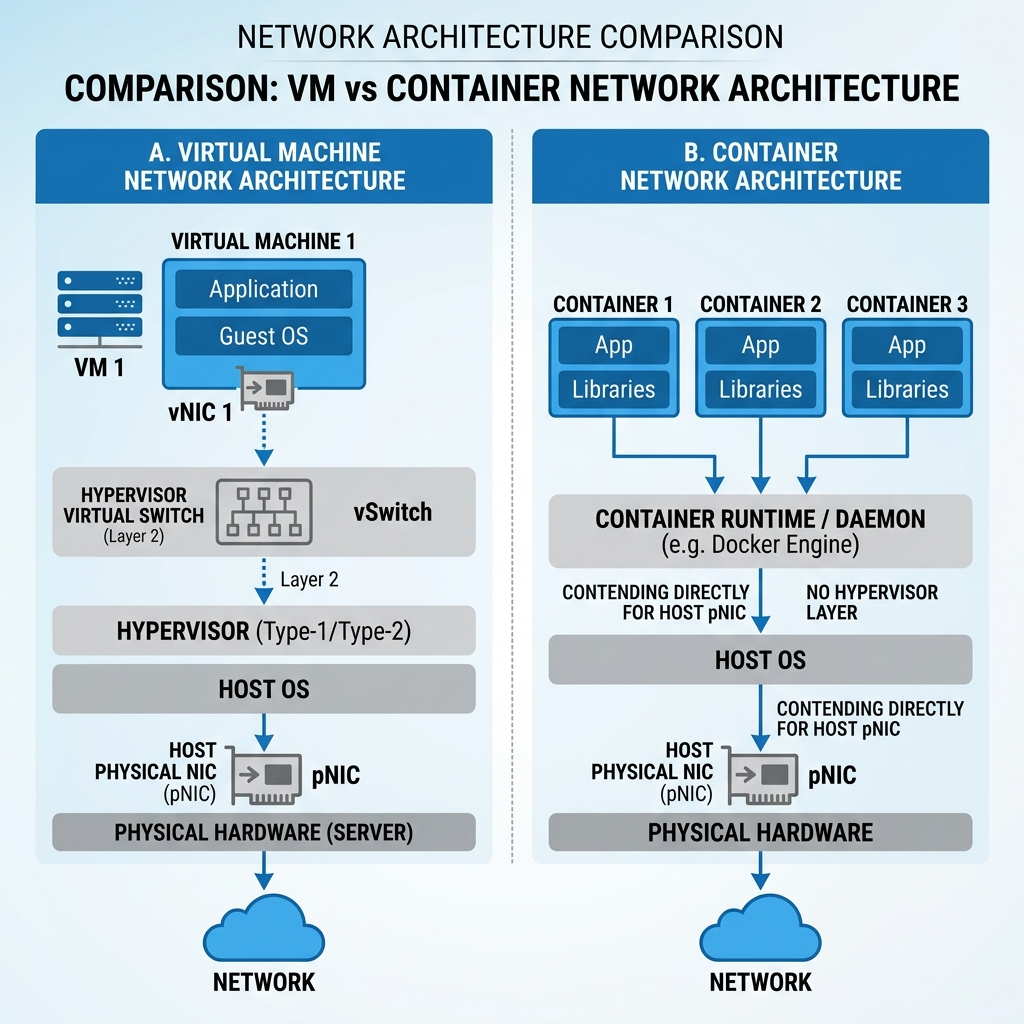
\includegraphics[width=0.8\textwidth]{images/container_vm_network.png}
    \caption{Architettura di rete: astrazione vNIC (VM) vs contesa e NAT (Container).}
\end{figure}

L'integrazione di Container e Virtualizzazione è però lo standard: il cloud esegue spesso cluster Kubernetes composti da \textit{Worker node} che sono essi stessi macchine virtuali, combinando così la leggerezza e facilità di deployment del container con il robusto isolamento hardware (evitando container escape) della VM.

\chapter{Cloud Computing, Orchestrazione e Sicurezza}

\section{Il Modello Cloud Computing}
\begin{figure}[H]
    \centering
    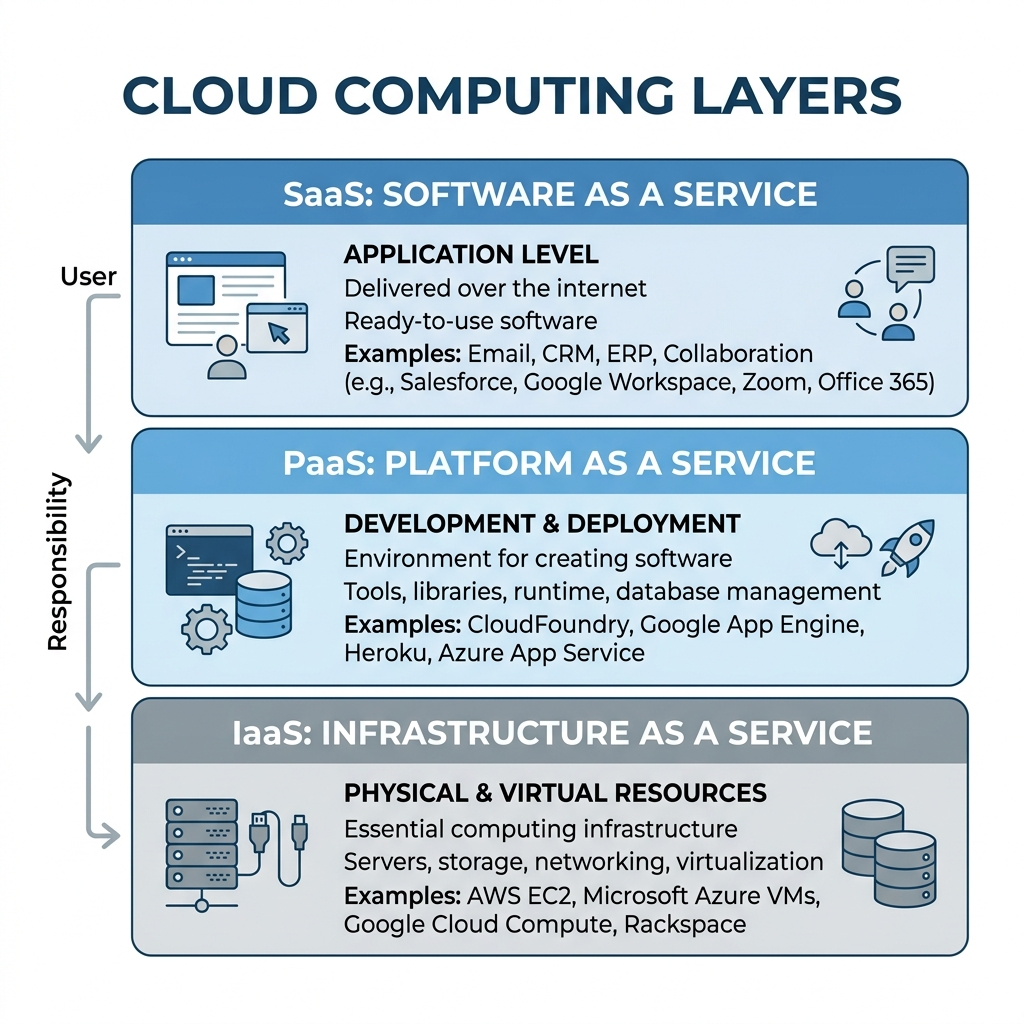
\includegraphics[width=0.8\textwidth]{images/cloud_computing.png}
    \caption{Rappresentazione astratta dei layer dell'architettura Cloud Computing.}
\end{figure}
Il cloud computing rappresenta non solo un cambio tecnologico, ma un profondo mutamento nel modello di business IT: si passa dall'acquisto di hardware (CapEx) al pagamento per consumo di un servizio (OpEx).

\begin{tipbox}[Le Sfide della Pubblica Amministrazione]
Costruire un cloud per un'azienda nativa digitale o per la Pubblica Amministrazione (PA) sono due sfide opposte. Una startup opera in ambiente \textbf{Greenfield} (si parte da zero con standard moderni). La PA opera tipicamente in \textbf{Brownfield}: deve migrare nel cloud applicativi e mainframe vecchi di decenni senza interrompere servizi critici ai cittadini. Inoltre subentrano ostacoli strutturali:
\begin{itemize}
    \item \textbf{Governance:} Modello centralizzato (più sicuro ed economico su scala nazionale) vs Federato (politicamente preferito dagli enti locali che non vogliono cedere il controllo sui propri dati).
    \item \textbf{Chargeback:} Come ripartire esattamente i costi (fatturazione interna) tra dipartimenti/ministeri diversi che condividono lo stesso hardware senza generare contenziosi.
    \item \textbf{Procurement:} L'acquisto di hardware fisico nei cloud on-premise della PA richiede estenuanti gare d'appalto pubbliche (con ritardi medi di 1-2 anni), rendendo il server acquistato già tecnologicamente obsoleto nel momento in cui viene fisicamente consegnato nel datacenter.
\end{itemize}
\end{tipbox}

\subsection{Definizione e Caratteristiche (NIST)}
Secondo il NIST, il cloud è caratterizzato da:
\begin{itemize}
    \item \textbf{On-demand self-service:} Provvigionamento autonomo da parte del cliente senza intervento umano del provider.
    \item \textbf{Broad network access:} Accessibilità ubiqua via rete standard.
    \item \textbf{Resource pooling:} Risorse condivise in modalità multi-tenant.
    \item \textbf{Rapid elasticity:} Capacità di scalare rapidamente verso l'alto e verso il basso (le risorse appaiono infinite al consumatore).
    \item \textbf{Measured service:} Modello pay-as-you-go e misurazione continua delle risorse.
\end{itemize}

\subsection{Modelli di Servizio}
\begin{itemize}
    \item \textbf{IaaS (Infrastructure as a Service):} Il provider fornisce CPU, rete e storage "grezzi" o virtualizzati. Il consumatore gestisce dal Sistema Operativo in su.
    \item \textbf{PaaS (Platform as a Service):} Il provider gestisce anche l'OS e l'ambiente di runtime. Il consumatore carica solo la sua applicazione (es. database managed, web app).
    \item \textbf{SaaS (Software as a Service):} Tutto è gestito dal provider (es. Gmail, Microsoft 365). L'utente usa solo il software finale.
\end{itemize}

\section{Architettura di Riferimento (Reference Model)}
Il Reference Model si articola in livelli (layer):
\begin{enumerate}
    \item \textbf{Physical Layer:} Hardware fisico (Server, Switch, Storage array). A questo livello operano gli \textbf{Element Manager}, ovvero interfacce di gestione proprietarie fornite dal produttore (es. la GUI di un singolo switch o di un array EMC) che vedono \textit{solo} il proprio dispositivo fisico.
    \item \textbf{Virtual Layer:} Macchine virtuali, vSwitch, LUN virtuali. Astrae l'hardware fisico fornendo pool di risorse flessibili.
    \item \textbf{Control Layer:} Si occupa di gestire e raggruppare globalmente le risorse virtuali. Qui opera lo \textbf{Unified Manager} (es. VMware vCenter o Microsoft SCVMM), un super-gestore che aggrega migliaia di host ignorando le differenze di brand hardware e permette all'amministratore di applicare \textit{policy} di allocazione (riserve assolute vs relative) e di sovra-allocazione (Overbooking).
    \item \textbf{Orchestration Layer:} Automatizza flussi di lavoro complessi tramite script e chiamate asincrone ad API. Mentre il control layer esegue un singolo compito primario ("accendi VM"), l'orchestratore coordina una \textit{pipeline} intera multi-step ("crea VM, configura vSwitch, alloca IP, installa OS, installa Database").
    \item \textbf{Service Layer:} Fornisce il \textit{Cloud Portal} e il \textit{Service Catalog} in modalità self-service, da cui gli utenti finali (tenant) ordinano le risorse con un click, senza dover aprire ticket all'IT.
\end{enumerate}

\subsection{Cloud Service Lifecycle}
Dietro le quinte, l'erogazione di un servizio cloud passa attraverso quattro macro-fasi obbligatorie:
\begin{itemize}
    \item \textbf{Phase 1: Service Planning.} L'architetto IT definisce i confini del servizio, calcola le risorse richieste e, soprattutto, definisce la \textbf{Billing Policy} (la metrica esatta di fatturazione, es. per GB allocato, per CPU-hour o per Giga di traffico in uscita).
    \item \textbf{Phase 2: Service Creation.} L'orchestratore riceve l'ordine dal portale e lo converte in dozzine di chiamate API concrete all'infrastruttura per costruire il servizio, allocando IP, dischi e CPU.
    \item \textbf{Phase 3: Service Operation.} Il servizio entra in produzione e passa in mano al tenant. Viene costantemente monitorato tramite sonde per verificare il rispetto degli SLA (Quality of Service) e per quantificare le risorse consumate a fini di addebito (Metering).
    \item \textbf{Phase 4: Service Termination.} Alla scadenza del contratto o disdetta, il sistema deve automaticamente disallocare tutte le risorse, cancellare i dati in modo irreversibile (Secure Wipe) per proteggere la privacy del vecchio tenant, e rimettere indirizzi IP e storage nel pool disponibile.
\end{itemize}

\begin{definitionbox}[SLA (Service Level Agreement) e Clausole Legali]
È il contratto vincolante tra cloud provider e consumatore che stabilisce i livelli di servizio garantiti (uptime, performance, security). Include metriche di misurazione e sanzioni (\textit{Service Credits}) in caso di violazione. Storicamente, gli SLA nascondono clausole complesse a favore del provider: 
\begin{itemize}
    \item \textbf{Downtime vs User-minutes:} Il calcolo del disservizio non è assoluto. Un guasto del 10\% dell'infrastruttura potrebbe non violare l'SLA se calcolato sul totale degli "user-minutes" mensili previsti.
    \item \textbf{Esclusioni:} Le manutenzioni programmate (\textit{Scheduled Downtime}) o i disservizi causati da un uso improprio del cliente esulano dalle sanzioni.
    \item \textbf{Lock-in:} Difficoltà tecnico-legali nel migrare i propri dati in uscita senza incorrere in enormi costi di trasferimento (\textit{Egress}) o dipendenza da formati proprietari.
\end{itemize}
\end{definitionbox}

\section{Business Continuity e Data Protection}
Il cloud assume che i guasti hardware siano fisiologici. L'obiettivo è minimizzare l'impatto sul servizio (High Availability).
I parametri principali sono:
\begin{itemize}
    \item \textbf{RTO (Recovery Time Objective):} Tempo necessario per ripristinare il servizio in caso di disastro.
    \item \textbf{RPO (Recovery Point Objective):} Quanto indietro nel tempo si perde in dati in caso di ripristino. Determina la frequenza dei backup.
\end{itemize}

\subsection{Tecniche di Resilienza e Limiti Geografici}
Per evitare i \textbf{SPOF (Single Point of Failure)}, si usano tecniche di ridondanza su più livelli:
\begin{itemize}
    \item \textbf{Failover di Servizio vs Replicazione VM:} Il \textit{Service Failover} tradizionale (es. Windows Server Failover Cluster) si basa su un nodo secondario passivo; se il primario muore, il secondario monta lo storage condiviso e fa un lento reboot a freddo dell'applicativo (con RTO di minuti). La \textit{Replica VM} o la \textbf{Continuous Data Protection (CDP)} operano invece a un livello inferiore. Un CDP inietta un driver (\textit{Write Splitter}) nell'hypervisor che biforca ogni scrittura I/O: una copia va al disco locale, l'altra via rete asincrona al sito di Disaster Recovery. Utilizza un \textit{Journal Volume} per mantenere una cronologia granulare al secondo, permettendo di "riavvolgere" nel tempo l'intera VM a 5 secondi prima di un eventuale attacco ransomware.
    \item \textbf{Active/Active vs Active/Passive:} L'approccio Active/Passive usa un nodo secondario in standby. L'approccio Active/Active distribuisce il carico simultaneamente su più datacenter geografici, ma incontra un grave limite fisico dettato dalla velocità della luce nella fibra ottica.
    \item \textbf{Replica Sincrona vs Asincrona:} Affinché due datacenter operino in vero Active/Active (senza corrompere i database condivisi), la replica dello storage deve essere \textbf{Sincrona} (la scrittura viene confermata al client solo dopo che entrambi i siti geografici l'hanno salvata). Per far ciò senza paralizzare le applicazioni, il tempo di latenza (\textit{Round-Trip Time}) tra i datacenter non deve superare i \textbf{10-15 millisecondi}, il che obbliga i siti a non distare più di $\sim$100-150 km l'uno dall'altro. Per distanze superiori (es. tra continenti), si è obbligati a usare la replica \textbf{Asincrona} (dove c'è una finestra di vulnerabilità, RPO > 0), poiché l'attesa del segnale luminoso renderebbe il sistema inutilizzabile.
    \item \textbf{Availability Zones:} Divisione in zone distinte (spesso in datacenter diversi entro la soglia dei 15ms) isolate da guasti comuni (alimentazione, allagamenti) ma connesse in fibra ottica dedicata (Dark fiber) per apparire come un'unica grande infrastruttura logica.
\end{itemize}

\subsection{Application Resiliency: Progettare per il Fallimento}
Le moderne architetture cloud si arrendono all'evidenza statistica che l'hardware fallirà inevitabilmente. La resilienza viene quindi astratta e spostata totalmente a livello software (\textbf{Design for Failure}):
\begin{itemize}
    \item \textbf{Statelessness e Persistent State:} I container e i web server non devono \textit{mai} salvare dati locali. Lo stato persistente viene scaricato costantemente su database esterni o Object Storage (es. S3), permettendo a Kubernetes di "uccidere" e ricreare un nodo applicativo infetto o guasto in 1 secondo, senza perdite e senza causare interruzioni agli utenti.
    \item \textbf{Graceful Degradation:} Se il sofisticato servizio di raccomandazione AI di Netflix fallisce nel cloud, l'interfaccia utente non deve generare una pagina di errore 500. Deve degradare l'esperienza in modo "elegante", servendo automaticamente una banale lista statica generica precompilata di film.
    \item \textbf{Retry Logic e Circuit Breaker:} Le chiamate API asincrone tra microservizi cloud falliranno per timeout di rete o latenza. Si implementano pattern software per ritentare (\textit{Exponential Backoff}) o "aprire il circuito" (\textit{Circuit Breaker}), disabilitando del tutto la chiamata problematica per evitare di bombardare e definitivamente abbattere un microservizio già congestionato.
    \item \textbf{Event-Driven Architecture:} Disaccoppiamento tramite code asincrone (es. Kafka o RabbitMQ). Se un database è temporaneamente sovraccarico per un picco di traffico imprevedibile, le scritture in arrivo si accumulano pazientemente in coda invece di fallire, venendo smaltite non appena il database torna a respirare.
\end{itemize}

\section{Sicurezza (Security)}
La sicurezza nel cloud si basa sul concetto di \textbf{Trust} tra cliente e fornitore, costruito tramite visibilità e controllo. L'obiettivo è garantire i pilastri \textbf{CIA} (Confidentiality, Integrity, Availability).

\subsection{Minacce Classiche e Attacchi}
Storicamente, i datacenter dovevano difendersi da attacchi mirati al perimetro (Firewall). Le minacce classiche includono:
\begin{itemize}
    \item \textbf{Spoofing:} Falsificazione dell'identità (es. IP spoofing) per bypassare le ACL.
    \item \textbf{Man-in-the-Middle (MitM) e Sniffing:} Intercettazione non autorizzata del traffico in transito.
    \item \textbf{Denial of Service (DDoS):} Saturazione delle risorse (computazionali o di banda) per abbattere la disponibilità del servizio.
    \item \textbf{Phishing / Social Engineering:} Compromissione del fattore umano per rubare credenziali valide.
\end{itemize}

\subsection{Gestione delle Identità e Policy (AAA e RBAC)}
Oltre alla difesa perimetrale, il fondamento vitale della sicurezza cloud in ambienti multi-tenant è la corretta gestione degli accessi e dei privilegi:
\begin{itemize}
    \item \textbf{Modello AAA:} Rappresenta il framework di sicurezza fondamentale.
    \begin{itemize}
        \item \textit{Authentication (Chi sei?):} Verifica rigorosa dell'identità (es. tramite password, certificati o Multi-Factor Authentication).
        \item \textit{Authorization (Cosa puoi fare?):} Valutazione e concessione dei permessi esatti dell'utente sulle singole risorse del cloud.
        \item \textit{Accounting (Cosa hai fatto?):} Tracciamento e logging immutabile di ogni azione (Audit Trail) per scopi di analisi forense post-incidente e per la fatturazione.
    \end{itemize}
    \item \textbf{RBAC (Role-Based Access Control):} Nel cloud i permessi non si assegnano quasi mai al singolo utente direttamente (sarebbe ingestibile). Vengono creati dei \textbf{Ruoli} logici (es. "Storage Admin", "Auditor"). L'utente assume il ruolo o viene associato ad esso. Questo sistema evita la proliferazione incontrollata di privilegi e garantisce il rispetto del principio della sicurezza del \textit{Least Privilege} (fornire sempre e solo il minimo privilegio necessario per compiere una mansione).
\end{itemize}

\subsection{Approccio Defense-in-Depth e Zero Trust}
Poiché gli attacchi classici hanno dimostrato che non esiste un solo perimetro sicuro e che le minacce provengono anche dall'interno (\textit{Insider Threat}), il modello classico (basato su un'unica DMZ esterna) è oggi sostituito dalla \textbf{Zero Trust Architecture (ZTA)}. Il principio è: "Non fidarsi mai, verificare sempre", basandosi su autenticazione forte e \textit{Micro-segmentazione} dinamica prima di accedere a ogni singolo workload.
La base dell'architettura di sicurezza è la \textbf{TCB (Trusted Computing Base)}, l'insieme dei componenti critici (es. hypervisor, firmware BMC), che se compromessi fanno cadere inevitabilmente l'intera catena di fiducia.

\subsection{Gestione dei Rischi (GRC)}
Si racchiude nel framework \textbf{GRC} (Governance, Risk management, Compliance):
\begin{itemize}
    \item Nessun sistema è inviolabile al 100\%. Il Risk Assessment valuta la probabilità di incidente contro il costo della contromisura.
    \item La Compliance assicura il rispetto di normative come GDPR, NIS2, ecc.
\end{itemize}

\chapter{Operations e Considerazioni Finali}

\section{Service Operations Management}
Questa fase chiude il ciclo di vita del datacenter affrontando la parte procedurale e operativa: tutto ciò che avviene \textit{dopo} che l'infrastruttura è in piedi. Mantenere funzionante un cloud significa garantire il rispetto degli \textbf{SLA (Service Level Agreement)}, identificare guasti, pianificare le risorse e tracciare ogni modifica.
Le attività principali si raggruppano in:
\begin{itemize}
    \item \textbf{Monitoring:} Osservare continuamente lo stato dell'infrastruttura e identificare anomalie.
    \item \textbf{Configuration e Change Management:} Tracciare l'inventario e governare ogni modifica al sistema.
    \item \textbf{Capacity Management:} Capire quante risorse serviranno nei prossimi mesi per approvvigionarle prima che si esauriscano.
    \item \textbf{Incident e Problem Management:} Rispondere a eventi non pianificati e prevenire la loro ricorrenza.
\end{itemize}

\subsection{Monitoring e Predictive Failure}
In un'infrastruttura moderna esistono milioni di contatori (rete, hypervisor, BMC). Poiché ogni sistema "pulito" genera migliaia di warning nei log, il vero lavoro del monitoring è separare i problemi reali dal rumore di fondo usando i dati storici.
Si distinguono:
\begin{itemize}
    \item \textbf{Configuration monitoring:} Rilevare modifiche non autorizzate o violazioni di policy.
    \item \textbf{Availability monitoring:} Verificare la raggiungibilità dei servizi e lo stato dei singoli componenti hardware (es. dischi).
    \item \textbf{Security monitoring:} Fondamentale nei cloud pubblici, monitora accessi logici e fisici (es. sensori biometrici alle porte).
\end{itemize}

Una funzionalità avanzata è la \textbf{Predictive Failure Analysis}: i BMC integrano modelli statistici e, analizzando i pattern di un disco, emettono un avviso \textit{prima} che si rompa. Questo permette di rimuoverlo dal pool, sostituirlo e reinserirlo senza alcun impatto sull'utente.
\begin{warningbox}[Il clock della ridondanza e gli effetti a cascata]
Quando un componente guasta, il "clock comincia a ticchettare": la ridondanza è ridotta e la sostituzione deve essere rapida. Un fallimento può inoltre generare un \textbf{effetto a cascata}: il carico spostato su altri nodi sani li sovraccarica, facendoli crollare a loro volta.
\end{warningbox}

\subsection{Capacity Monitoring e Management}
Il Capacity Management ragiona come una compagnia assicurativa: si fanno stime statistiche e si scommette che non tutti useranno le risorse al massimo contemporaneamente. Questo permette la pratica dell'\textbf{Overbooking} (o \textit{over-commitment} di CPU e rete).
Alcune tecniche operative includono:
\begin{itemize}
    \item \textbf{Dynamic scheduling:} Bilanciamento automatico del carico tra le vCPU dei server fisici.
    \item \textbf{Tiering dello storage:} Spostare i dischi delle VM spente su storage lento ed economico. Alla riaccensione, la VM viene avviata e lo storage subisce una live migration in backgroud verso un tier veloce in modo totalmente trasparente per l'utente.
\end{itemize}

\section{Gestione dei Cambiamenti e dei Guasti}

\subsection{Change Management}
È il processo volto a registrare ogni singola modifica alla configurazione di un sistema nel \textbf{CMDB (Configuration Management Database)}. Quando qualcosa si rompe, la prima domanda del team operations è sempre "chi ha toccato qualcosa?". Qualsiasi modifica strutturale (es. aggiornamento DB) richiede un processo rigido: creazione di uno snapshot (garantendo la reversibilità in caso di rollback), aggiornamento, verifica e, solo se ha successo, eliminazione dello snapshot per non gravare sulle performance di I/O future a causa della catena dei file differenziali.

\subsection{Incident vs. Problem Management}
La distinzione ITIL tra incidente e problema è vitale per le operations:
\begin{definitionbox}[Incidente vs Problema]
Un \textbf{Incidente} è un evento non pianificato che degrada un servizio (approccio \textit{reattivo}: si risolve il sintomo nel minor tempo possibile).
Un \textbf{Problema} è la causa radice di uno o più incidenti (approccio \textit{proattivo}: si elimina la causa per evitare che si ripeta).
\end{definitionbox}
Esempio pratico: un disco si rompe e un pool di storage si esaurisce (incidente). Cambiare il disco risolve l'incidente. Il \textit{problem management} indaga e scopre che il pool era già troppo saturo, quindi la soluzione a lungo termine è espandere la capacità generale del cluster per prevenire guasti futuri.

\section{Considerazioni Finali sul Datacenter}
L'evoluzione dell'IT ha seguito un percorso che parte dalle basi fisiche (energia, dissipazione) fino all'astrazione totale (cloud). Alcuni concetti chiave riassuntivi:
\begin{itemize}
    \item \textbf{Il principio del bilanciamento:} Un sistema efficiente non è quello con il miglior componente assoluto, ma quello bilanciato. Una CPU iperveloce con uno storage a dischi meccanici darà un sistema lento. Il design del datacenter è per sua natura un esercizio per evitare e gestire i colli di bottiglia.
    \item \textbf{Workload divergence:} Mentre un tempo l'hardware era "general-purpose", oggi i carichi divergono. L'Intelligenza Artificiale richiede enormi quantità di memoria, GPU densamente impacchettate e latenze di rete ultra-basse, portando a concentrazioni di potenza termica (fino a gigawatt in singoli edifici) e soluzioni estreme di direct-to-chip liquid cooling impensabili un decennio fa.
    \item \textbf{Architettare per il carico:} Di fronte a enormi flussi di dati (es. gli esperimenti del CERN che producono 10 TB/s ma ne scartano il 90\% dopo una prima elaborazione), l'ingegnere deve dimensionare frontend e backend in modo asimmetrico, scegliendo l'infrastruttura (SAN vs Object/NAS) in base ai reali pattern di accesso, latenza accettabile e parallelismo richiesto.
\end{itemize}


\backmatter
% Eventuale bibliografia o glossario finale

\end{document}
